\documentclass[dissertation,copyright]{uathesis}
\usepackage[]{graphicx}\usepackage[]{color}
%% maxwidth is the original width if it is less than linewidth
%% otherwise use linewidth (to make sure the graphics do not exceed the margin)
\makeatletter
\def\maxwidth{ %
  \ifdim\Gin@nat@width>\linewidth
    \linewidth
  \else
    \Gin@nat@width
  \fi
}
\makeatother

\definecolor{fgcolor}{rgb}{0.345, 0.345, 0.345}
\newcommand{\hlnum}[1]{\textcolor[rgb]{0.686,0.059,0.569}{#1}}%
\newcommand{\hlstr}[1]{\textcolor[rgb]{0.192,0.494,0.8}{#1}}%
\newcommand{\hlcom}[1]{\textcolor[rgb]{0.678,0.584,0.686}{\textit{#1}}}%
\newcommand{\hlopt}[1]{\textcolor[rgb]{0,0,0}{#1}}%
\newcommand{\hlstd}[1]{\textcolor[rgb]{0.345,0.345,0.345}{#1}}%
\newcommand{\hlkwa}[1]{\textcolor[rgb]{0.161,0.373,0.58}{\textbf{#1}}}%
\newcommand{\hlkwb}[1]{\textcolor[rgb]{0.69,0.353,0.396}{#1}}%
\newcommand{\hlkwc}[1]{\textcolor[rgb]{0.333,0.667,0.333}{#1}}%
\newcommand{\hlkwd}[1]{\textcolor[rgb]{0.737,0.353,0.396}{\textbf{#1}}}%
\let\hlipl\hlkwb

\usepackage{framed}
\makeatletter
\newenvironment{kframe}{%
 \def\at@end@of@kframe{}%
 \ifinner\ifhmode%
  \def\at@end@of@kframe{\end{minipage}}%
  \begin{minipage}{\columnwidth}%
 \fi\fi%
 \def\FrameCommand##1{\hskip\@totalleftmargin \hskip-\fboxsep
 \colorbox{shadecolor}{##1}\hskip-\fboxsep
     % There is no \\@totalrightmargin, so:
     \hskip-\linewidth \hskip-\@totalleftmargin \hskip\columnwidth}%
 \MakeFramed {\advance\hsize-\width
   \@totalleftmargin\z@ \linewidth\hsize
   \@setminipage}}%
 {\par\unskip\endMakeFramed%
 \at@end@of@kframe}
\makeatother

\definecolor{shadecolor}{rgb}{.97, .97, .97}
\definecolor{messagecolor}{rgb}{0, 0, 0}
\definecolor{warningcolor}{rgb}{1, 0, 1}
\definecolor{errorcolor}{rgb}{1, 0, 0}
\newenvironment{knitrout}{}{} % an empty environment to be redefined in TeX

\usepackage{alltt}
\newcommand{\SweaveOpts}[1]{}  % do not interfere with LaTeX
\newcommand{\SweaveInput}[1]{} % because they are not real TeX commands
\newcommand{\Sexpr}[1]{}       % will only be parsed by R


%\documentclass[dissertation,CC-BY]{uathesis}
%\documentclass[dissertation,CC-BY-SA]{uathesis}
%documentclass[dissertation,CC-BY-ND]{uathesis}
%\documentclass[thesis]{uathesis}
%\documentclass[document]{uathesis}

% Package Usage
% These are the packages that we need
\usepackage{booktabs}
\usepackage{graphicx}
\usepackage{natbib}			% natbib is available on most systems, and is
					% terribly handy.
					
%May need to remove! Trying to fix nocite{*} biblography problem:
					% If you want to use a different Bibliography package, 
					% you should be able to, just change this
					% and the \bibliographystyle command below.  Be warned
					% that you may need to do a little hacking to get
					% the REFERENCES item to show up in your TOC.

% Compatibility with the AASTEX package 
% of the American Astronomical Society.
%\usepackage{deluxetable}		% Allows use of AASTEX deluxe tables
%\usepackage{aastex_hack}		% Allows other AASTEX functionality.

% These are other packages that you might find useful.
% For controlling the fonts, see
% http://www.math.uiuc.edu/~hartke/computer/latex/survey/survey.html
% The following is a nice font set:
%\usepackage{mathtime}			% Times for letters; Belleek math.
%
\usepackage{wrapfig}

\newenvironment{lydiawrapfigure}
 {%
%  \setlength{\intextsep}{0pt}% <--- Wrong!
  \setlength{\columnsep}{15pt}%
  \wrapfloat{figure}%
 }
 {\endwrapfloat}
 
 
\usepackage{caption}
\usepackage{subcaption}
\usepackage{tipa}
\usepackage{color,soul}
\usepackage{url}
\usepackage{blindtext}
\usepackage[inline]{enumitem}
\usepackage{breakurl}
\usepackage{mathtools}
\usepackage{amsmath}			% AMS Math (advanced math typesetting)
%\usepackage{lscape}			% Used for making fitting large tables in by putting them landscape
%\usepackage{refs}			
%
% If you are using hyper-ref (recommended), this command must go after all 
% other package inclusions (from the hyperref package documentation).
% The purpose of hyperref is to make the PDF created extensively
% cross-referenced.

%Also works! Change dvips to driverfallback=dvips.
\usepackage[driverfallback=dvips,bookmarks,colorlinks=true,urlcolor=black,linkcolor=black,citecolor=black]{hyperref}


%Works!
%\usepackage[pdftex,bookmarks,colorlinks=true,urlcolor=black,linkcolor=black,citecolor=black]{hyperref}
%HERE IS THE THING THAT NEEDS TO CHANGE TO GET LATEX TO WORK WITH RSTUDIO. USE pdftex instead of dvips.

% Set up some values.
\completetitle{Working Title: Ear Recorded Speech: A novel approach to automatic and human speech recognition}
\fullname{Samuel John Charles Johnston}			% Grad college wants your full name here.
\degreename{Doctor of Philosophy}	% Title of your degree.



\begin{document}
%set_parent(‘/Users/mwilli/Documents/Spring_2017/Dissertation_Document/Dissertation_Working_Directory_Draft/Dissertation_Main.Rnw')


 



\chapter{Human Speech Perception of Ear-Recorded speech\label{chapter4}}


\section{Introduction}

In order to judge the usefulness and intelligibility of the modified sounds recorded at the ear, it is necessary to run a human perception task on the recorded sounds.  Of primary interest is whether the speech recorded at the ear in a noisy condition a) has resulted in a sufficient reduction in the ambient noise level, and b) is markedly more intelligible that speech recorded at the \textit{mouth} in a noisy condition.

\section{Background}

% I need to demonstrate:
%   - Explaining the acoustic structure of speech in noise
%   - Demonstrating why speech in noise is difficult for humans to understand (mechanically? neurologically?)
%   - Explain the average/expected performance of Humans when recognizing speech in noise
%   - Show the variability in ability to understand speech in noise by different speakers.
The inability for human listeners to understand speech occurs from an information loss that can be due to a host of factors.  For example, information can be lost in the domain of time (eg. an intermittent signal), or from loss of intensity (eg. due to distance of the source), as well as the distortion of the source itself, such as a speech deficit (\cite{mattys:12}).  Of particular interest to the present study is the difficulty for human listeners to perfectly understand a speech signal due to additive background noise from different sources other than the desired speech signal.

The ability of the human auditory system to hear and differentiate multiple sources of sound from a single pressure wave is often given the term ``auditory scene analysis'' (\cite{bregman:94}).  The term ``scene analysis'' is borrowed from the visual domain, implying the separation of an ``scene'' (be it auditory or visual) into its component objects (again, be they auditory or visual). For the purposes of this study, we will be discussing human auditory ability to find multiple sound sources from a temporal stream of air pressure fluctuations (ie. sound) reaching the tympanic membrane.

To visualize the auditory scene, note the waveform (ie. the graph of air pressure fluctuations) that reaches the tympanic membrane, eg. see Figure \ref{fig:animal_singlechannel}.  It is composed of all environmental sounds contributing to the air pressure fluctuation at the tympanic membrane\footnote{Note that this is for illustration purposes; the waveform will obviously look different when shaped by a given environment and the human ear canal before reaching the tympanic membrane.}.
%
\begin{wrapfigure}{r}{0.5\textwidth}
\centering
  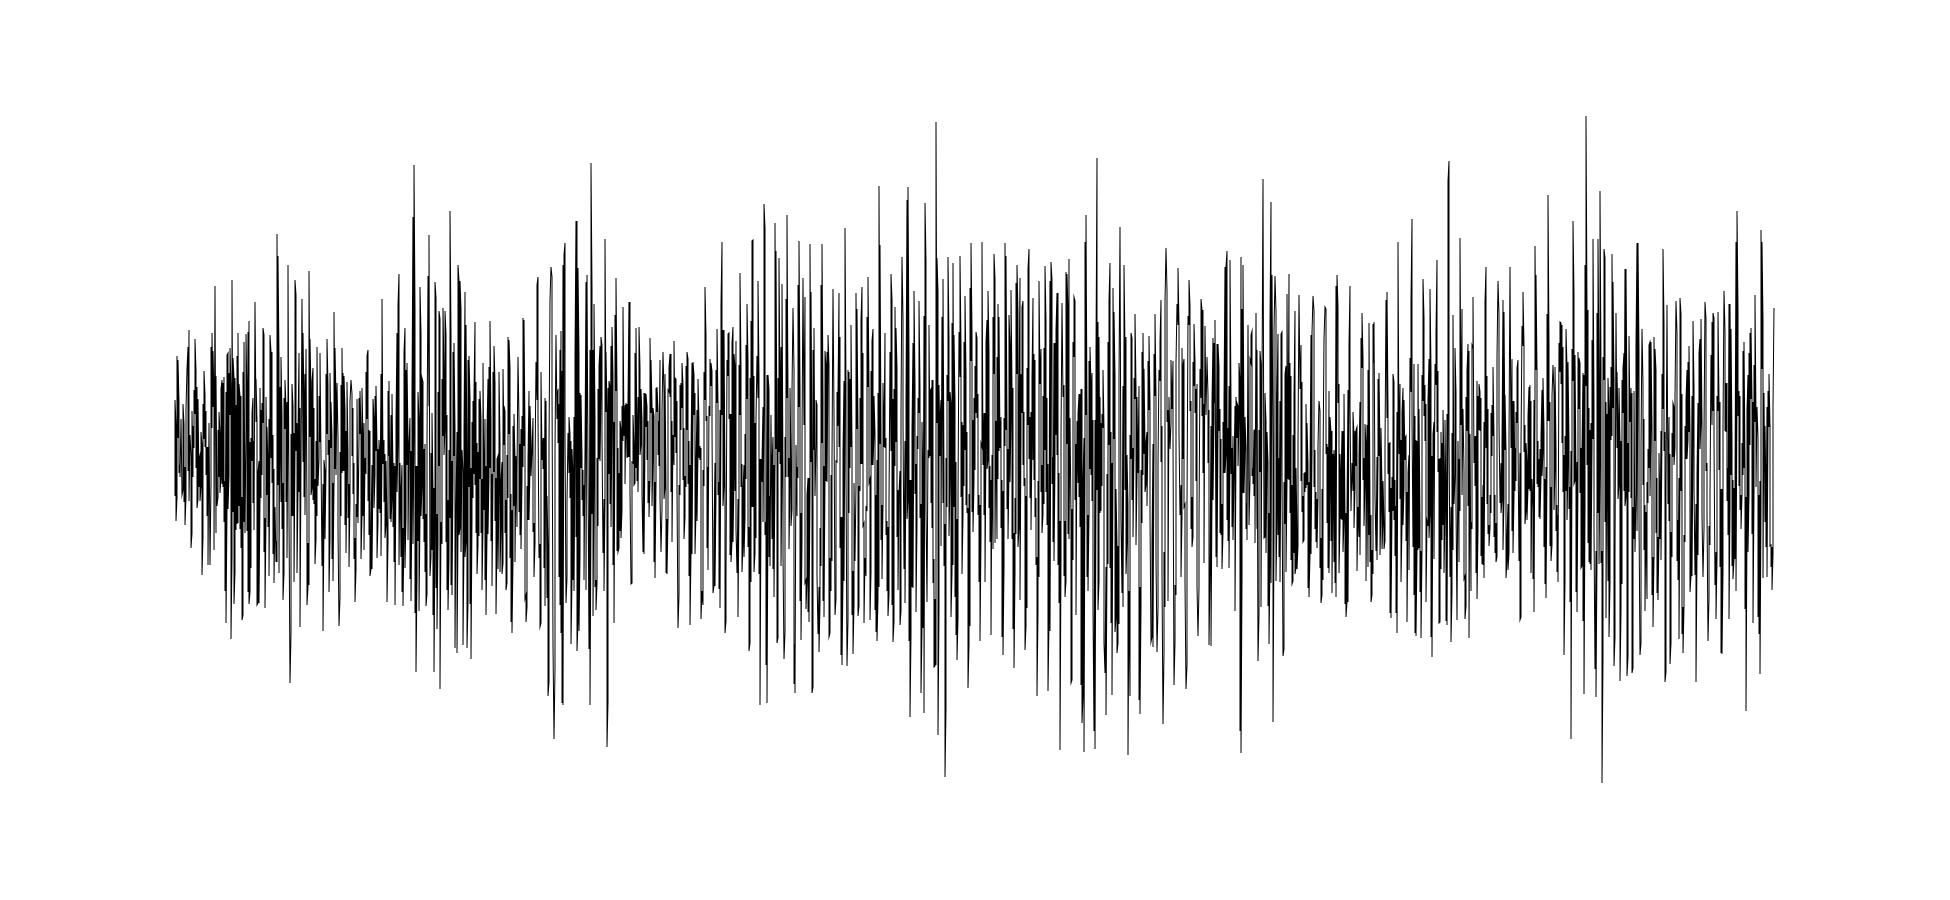
\includegraphics[width=0.45\textwidth]{figure/single-channel-animals.png}
  \caption{A waveform composed of multiple sound sources (cf. Fig. \ref{fig:animal_multichannel}.}
  \label{fig:animal_singlechannel}
\end{wrapfigure}

However, under the framework of auditory scene analysis, the human auditory system is able to separate this input signal into its various sources, or ``auditory objects''.  In effect, this would separate the above waveform into its actual component sources of human speech, and the sounds of a sheep, cow, and horse, seen in Figure \ref{fig:animal_multichannel}; ``The normal auditory system exhibits a remarkable ability to parse these complex scenes'' (\cite{middlebrooks:17}, 2).
%
\begin{figure}
\centering
  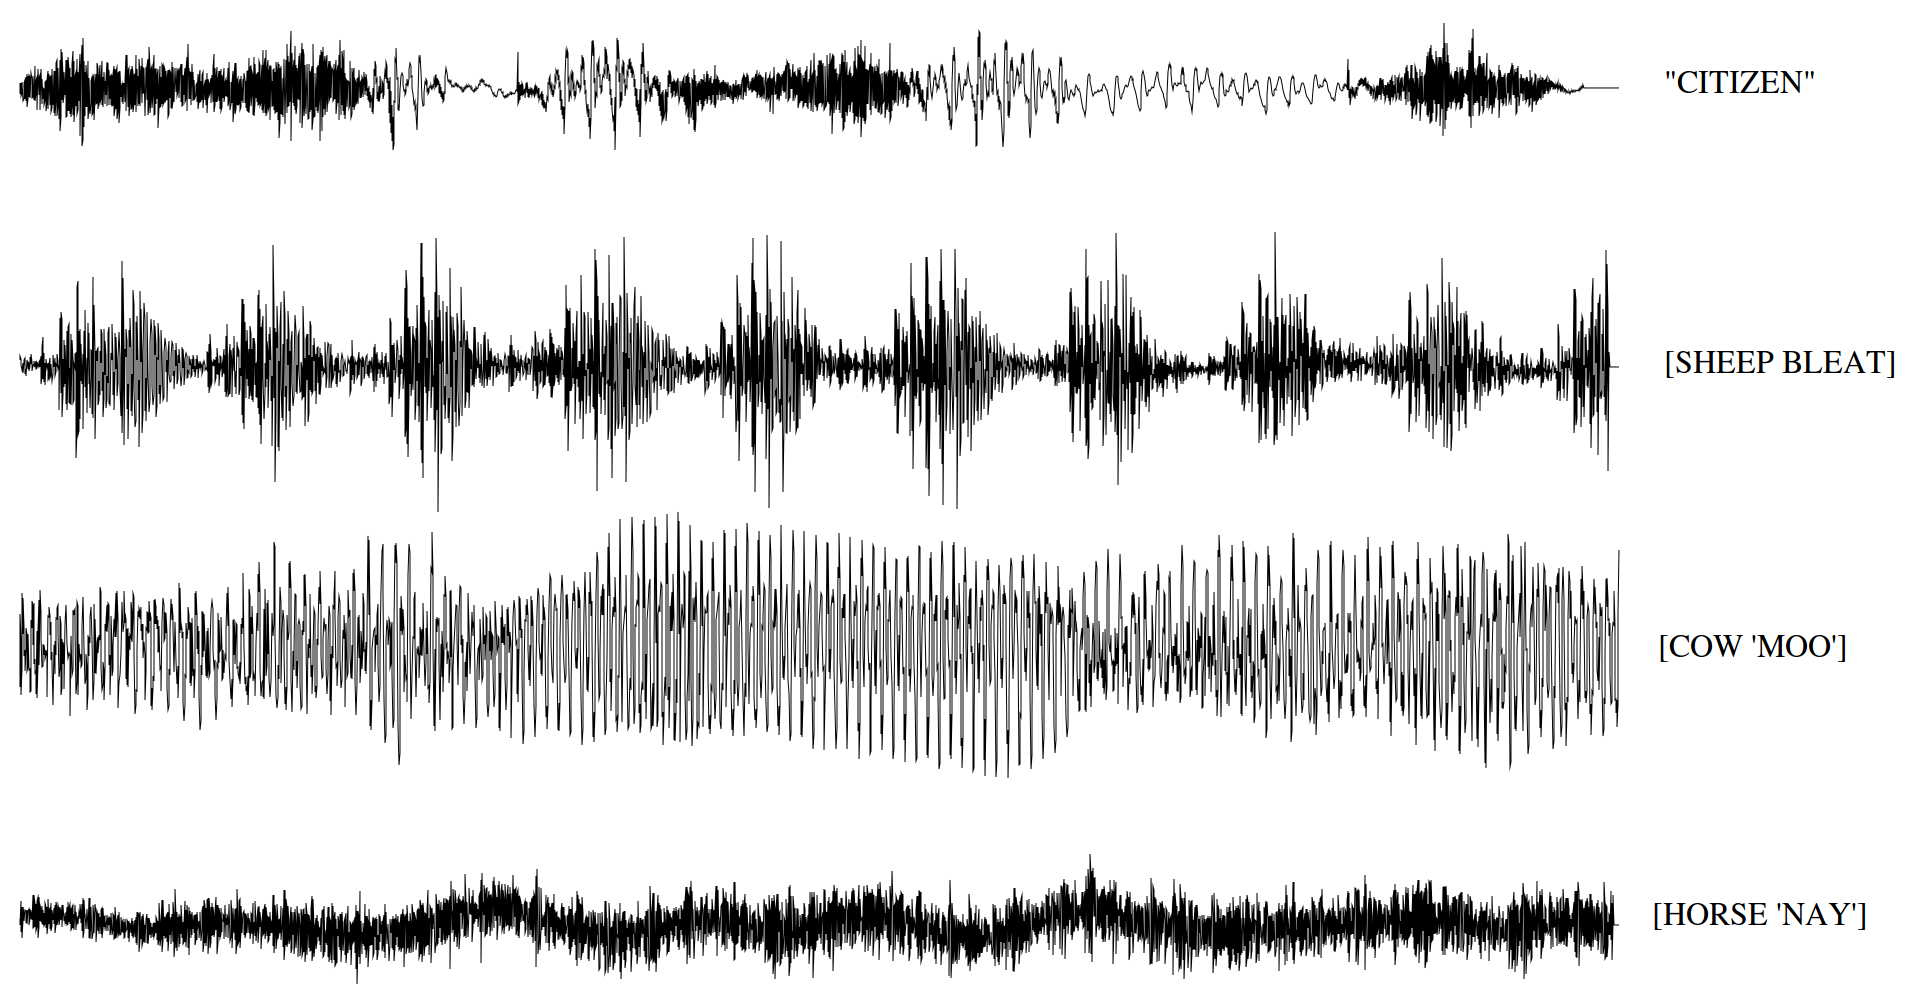
\includegraphics[width=0.95\textwidth]{figure/multi-channel-animals_w-text.png}
  \caption{The four component waveforms (human speech, sheep, cow, horse), of the combined waveform seen in Figure \ref{fig:animal_singlechannel}.}
  \label{fig:animal_multichannel}
\end{figure}
%
Of course, there reaches a point at which the auditory system fails and can no longer differentiate all sources, or, more relevant to this paper, recognize the information in a human speech signal when embedded with background noise from one or more additional sources.  The following section will describe in more depth the acoustics of speech in noise.
  
\subsection{Acoustics of Speech in Noise}

Speech in noise can be intuitively grouped into two components, the speech (more specifically the voice one is intending to hear) and the noise, called the ``masking'' element.  Broadly, masking can be defined as ``the process by which the threshold of hearing for one sound is raised by the presence of another'' (\cite{ansi:13}, 61).  This masking element is anything \textit{but} the voice\footnote{For the purposes of this paper, the term ``voice'' will be used throughout to refer to the singular speech source the listener desires to hear out of the masked signal.} (speech signal) that one is interested in.
%which, as indicated in Chapter 2\ref{chapter2}, could be of any form or loudness.

The masking process can be broken down into two forms: energetic masking and informational masking.  Energetic masking occurs when the masking element shares the same temporal and frequency elements of the voice.  It can be thought of as if the masked element and the voice are competing for ``space'' along the basilar membrane and then the auditory nerve (\cite{brungart:01}), but can also be considered to be competing for the listener's attention (ie. the listener must concentrate on ignoring the mask, and exclusively listening to the target, \cite{mattys:12}).  Energetic masking is normally thought to occur primarily in the ``lower'' auditory processes, eg. the cochlea and auditory nerve, though this is not always the case, as described further below.  

Informational masking can be broadly thought of as difficulties relating to memory, linguistic processing, and the like, oftentimes generalized to speech-on-speech noise.  This can even be restricted to cases in which the masking speech is intelligible speech, as \cite{mattys:10} failed to find informational masking in a cross-linguistic task. This is thought to occur primarily in the ``higher auditory processes'' in the brain.

This can be visualized in a diagram of overlapping speech presented in \cite{middlebrooks:17}, as seen in Figure \ref{fig:sos-masked-spctgrms}.
%
\begin{figure}
\centering
  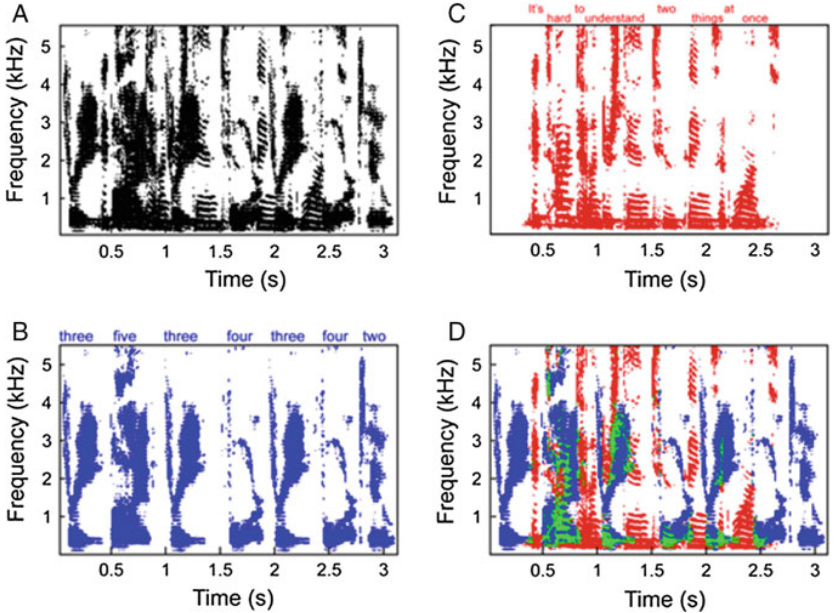
\includegraphics[width=0.95\textwidth]{figure/speech-on-speech_masked_spectrograms.png}
  \caption{Diagrams of different spectograms. (A) The spectogram of two temporally overlapping spoken utterances. (B) The spectogram of the utterance ``three five three four three four two.'' colored in blue (C) The spectogram of the sentence ``It's hard to understand two things at once.'' colored in red. (D) The overlap of the two spectograms (B) and (C), with the color green highlighting the areas of energy in frequency and time that overlap. }
  \label{fig:sos-masked-spctgrms}
\end{figure}
%
Say that utterance (C) in the figure is the desired ``voice'', leaving utterance (B) the masking element.  In (D), one can see the voice (red), the areas of direct frequency and temporal overlap in green, and in blue the remainder of the masking speech (B). This could primarily be viewed as a form of energetic masking (competition for lower-level processing), though upper level processing is required to take meaning from the desired voice, which is masked informationally by the other, competing voice carrying it's own information.

The five different background noises used in the study described in Chapter 2\ref{chapter2} primarily serve the purpose of energetic masking of the voice in the signal.  A small (5 second) portion of the spectrogram of each sound can be seen in Figure \ref{fig:bckgrnd-noises}.  These sounds don't produce any informational content themselves which mask the desired voice (the `cafe' noise, seen in Figure \ref{fig:spctgrm-cafe-background}, does contain speech babble, none of it intelligible), and so masking occurs by producing energy at the same time as - and in the same frequency range as - the recorded voice.
%
\begin{figure}
\begin{subfigure}{0.5\textwidth}
  \centering
  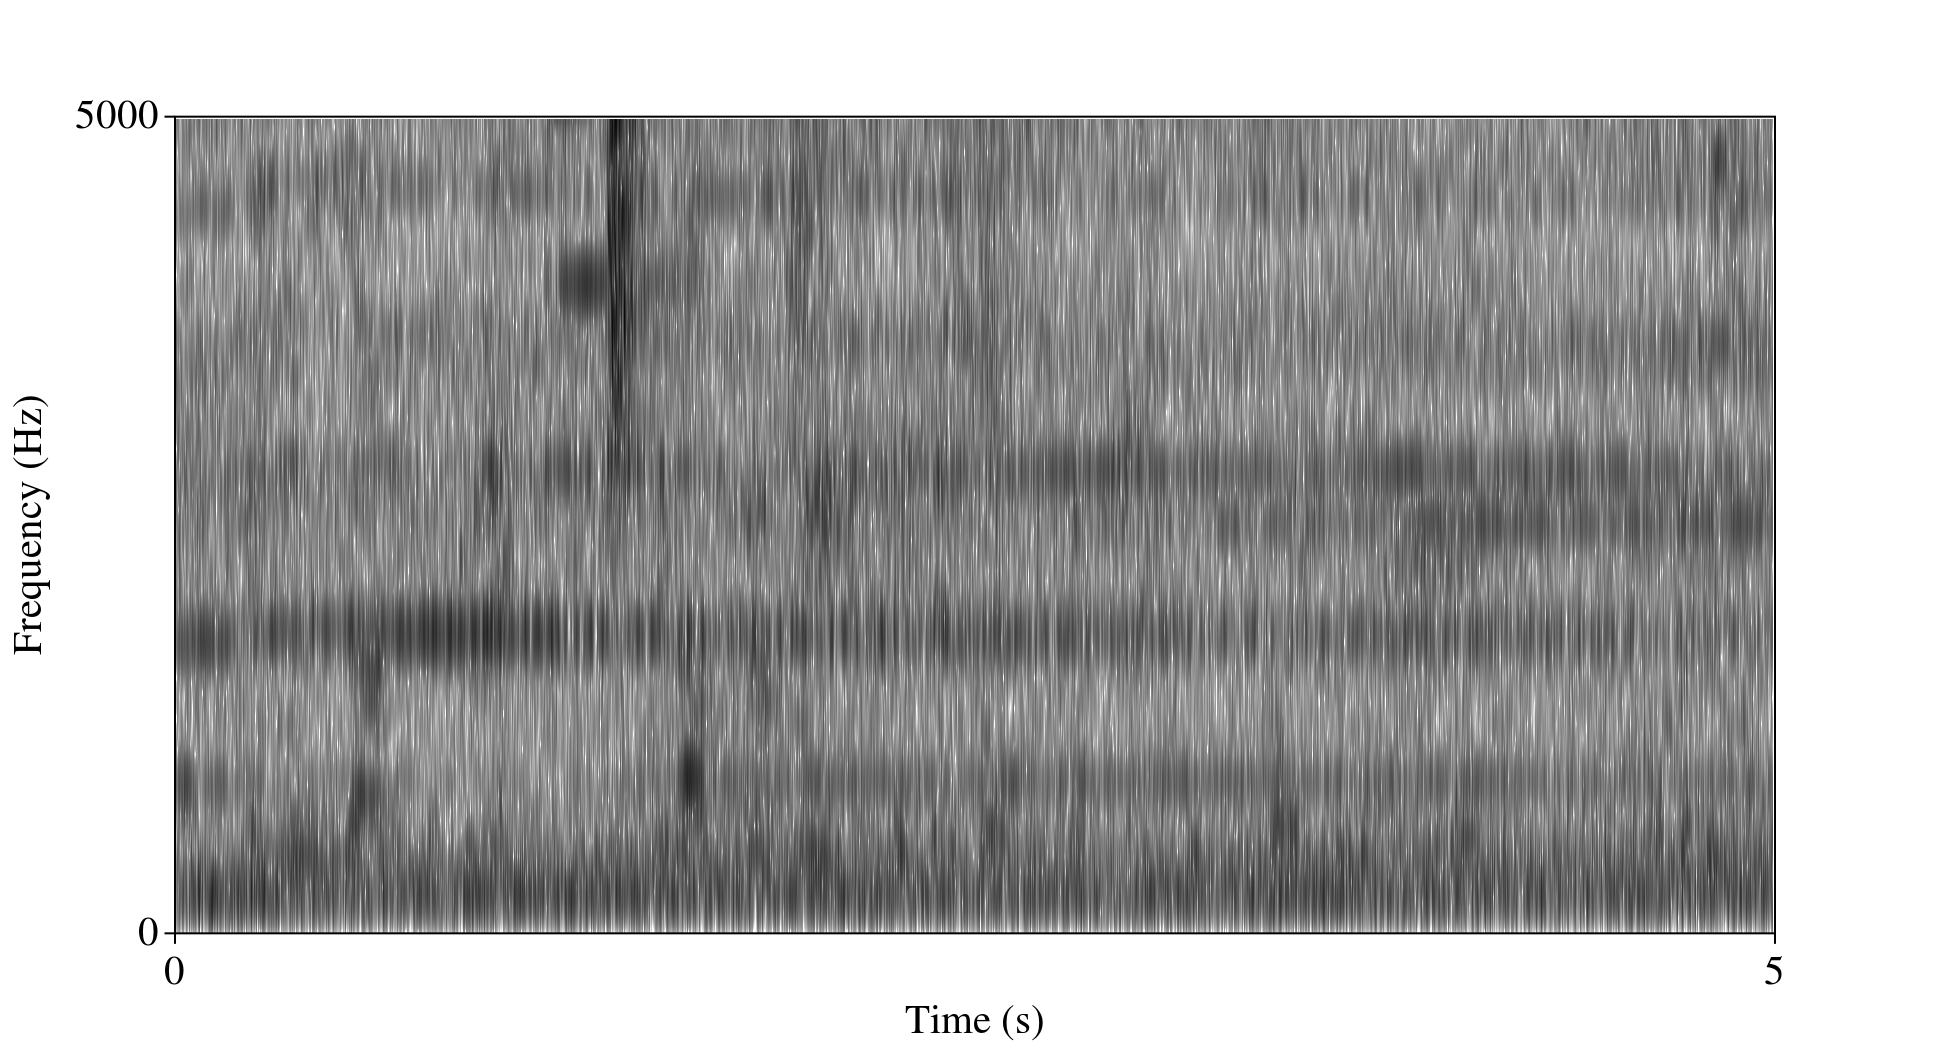
\includegraphics[width=0.9\textwidth]{figure/spctgrm-bus-background.png}
  \caption{Bus background noise.}
  \label{fig:bus-bkgrnd}
\end{subfigure}
\begin{subfigure}{0.5\textwidth}
  \centering
  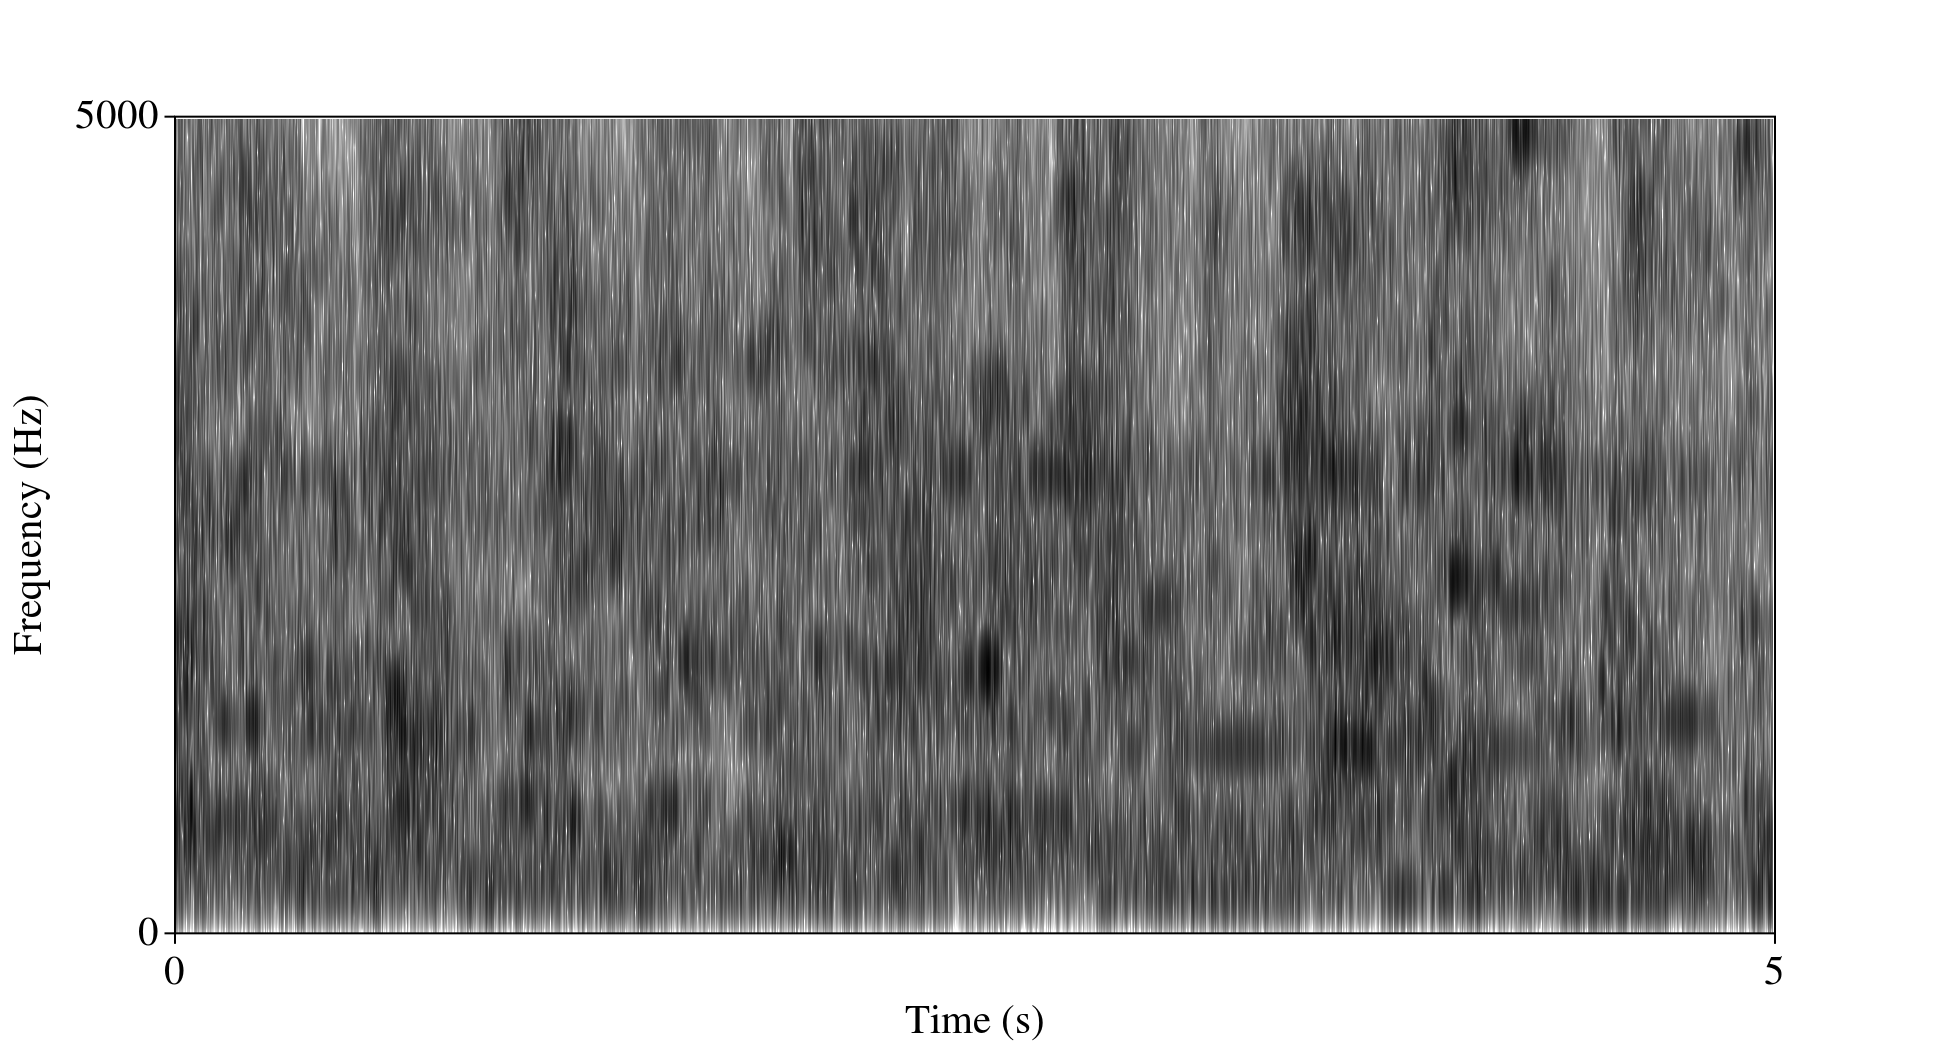
\includegraphics[width=0.9\textwidth]{figure/spctgrm-cafe-background.png}
  \caption{Cafe background noise.}
  \label{fig:cafe-bkgrnd}
\end{subfigure}%
\hfill
\begin{subfigure}{0.5\textwidth}
  \centering
  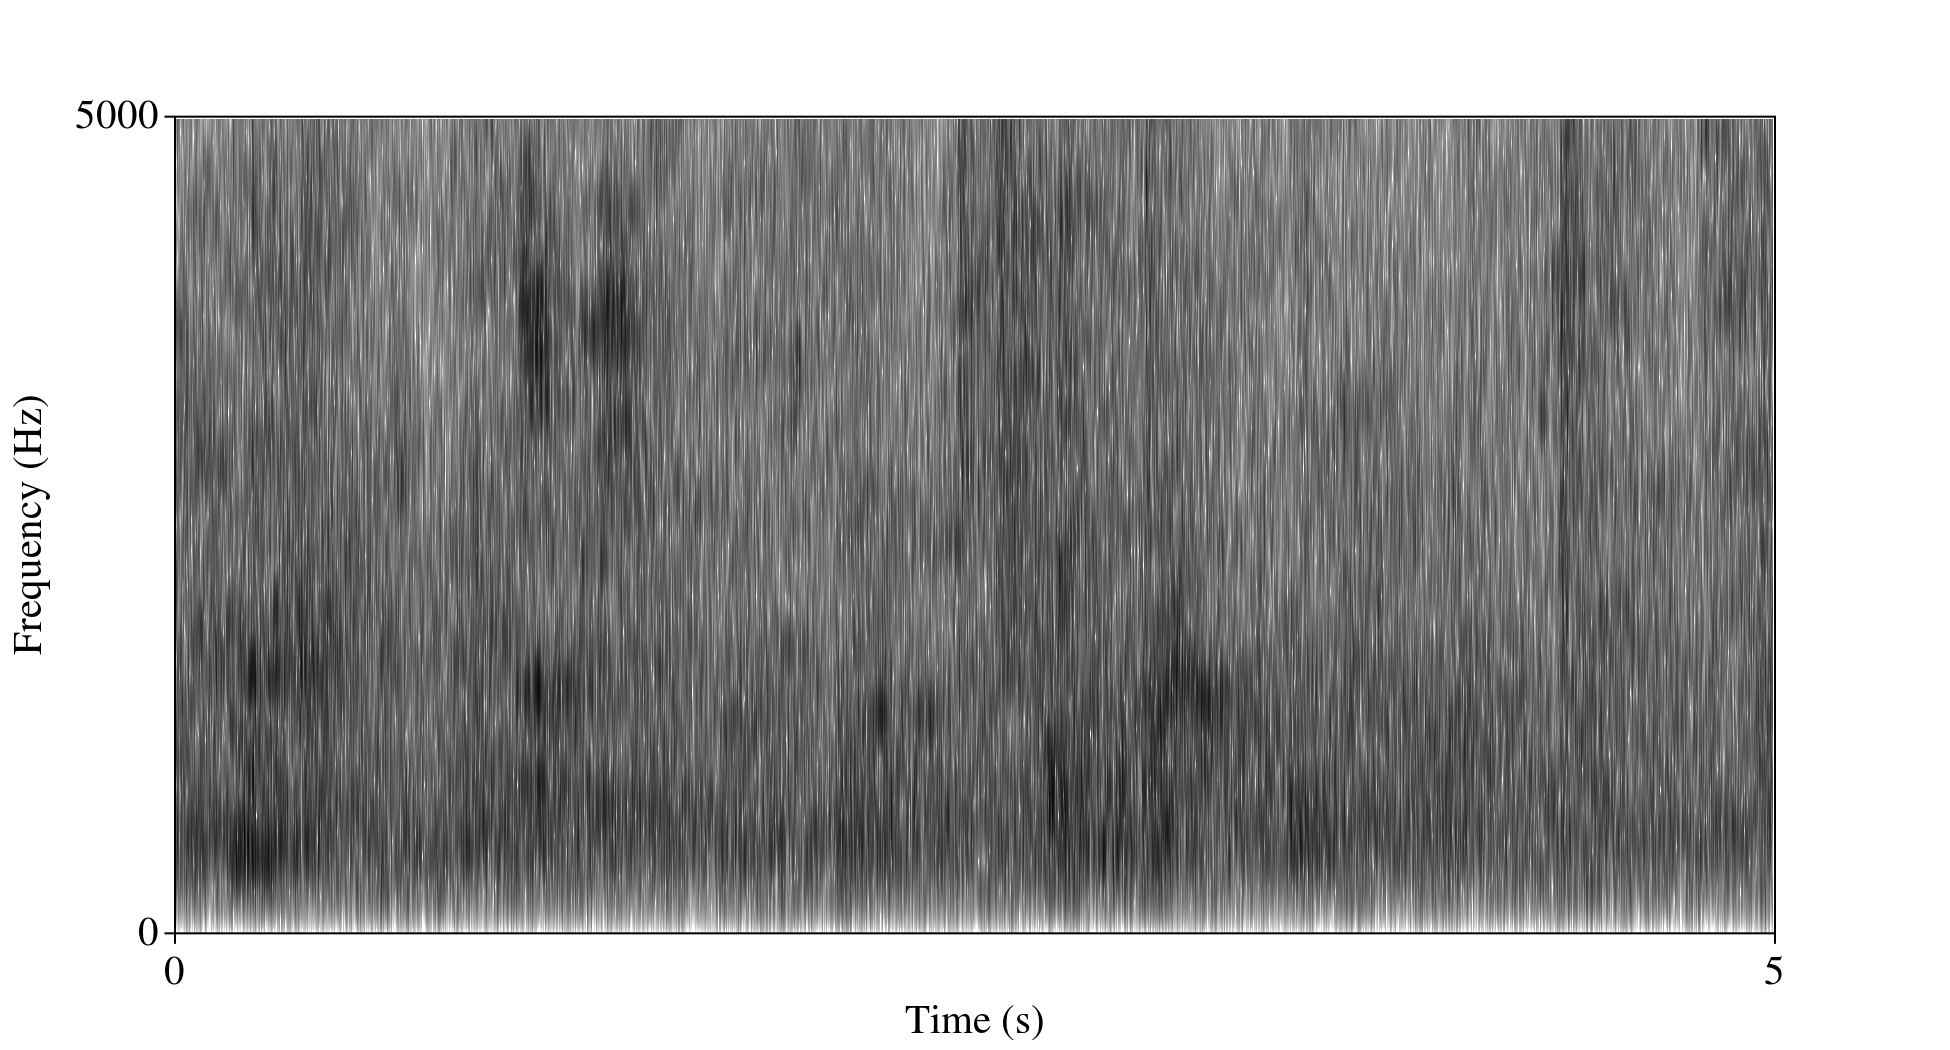
\includegraphics[width=0.9\textwidth]{figure/spctgrm-ped-background.png}
  \caption{Pedestrian background noise.}
  \label{fig:ped-bkgrnd}
\end{subfigure}
\begin{subfigure}{0.5\textwidth}
  \centering
  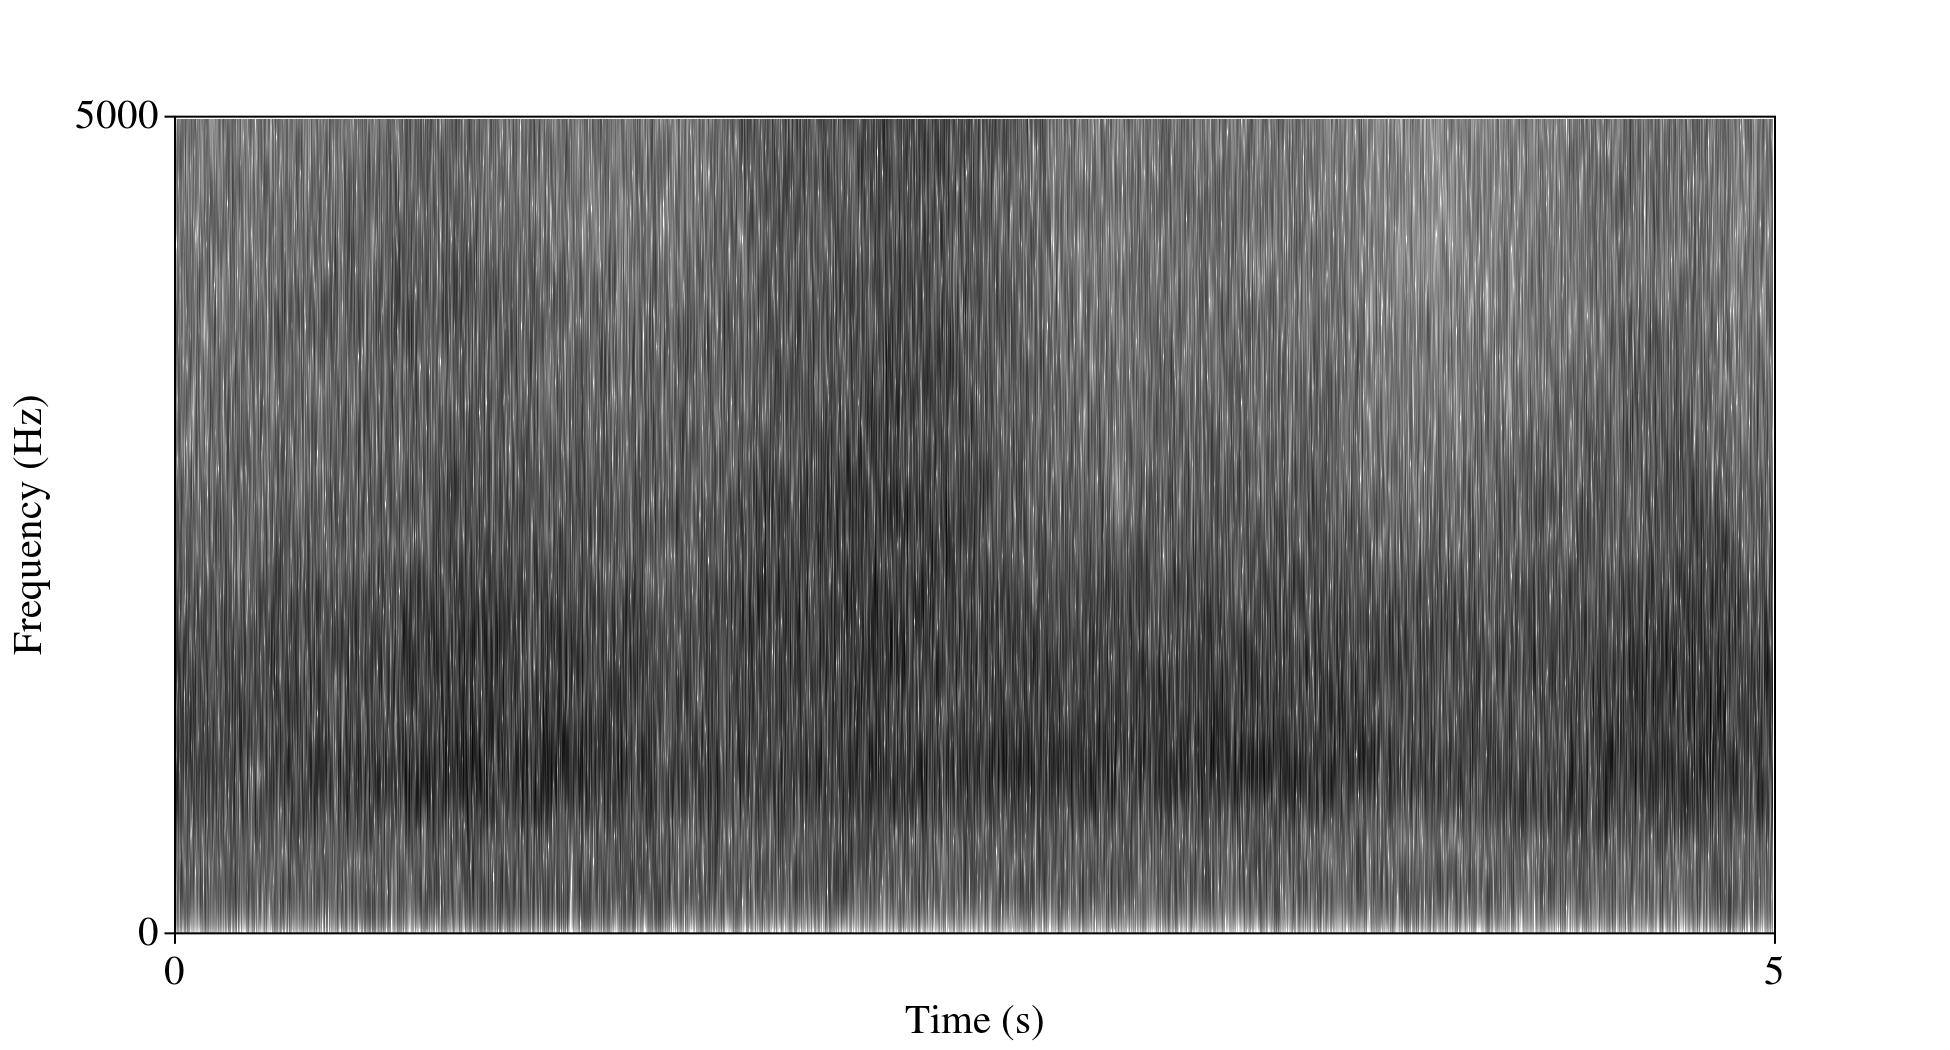
\includegraphics[width=0.9\textwidth]{figure/spctgrm-str-background.png}
  \caption{Street background noise.}
  \label{fig:str-bkgrnd}
\end{subfigure}%
\hfill
\begin{subfigure}{0.5\textwidth}
  \centering
  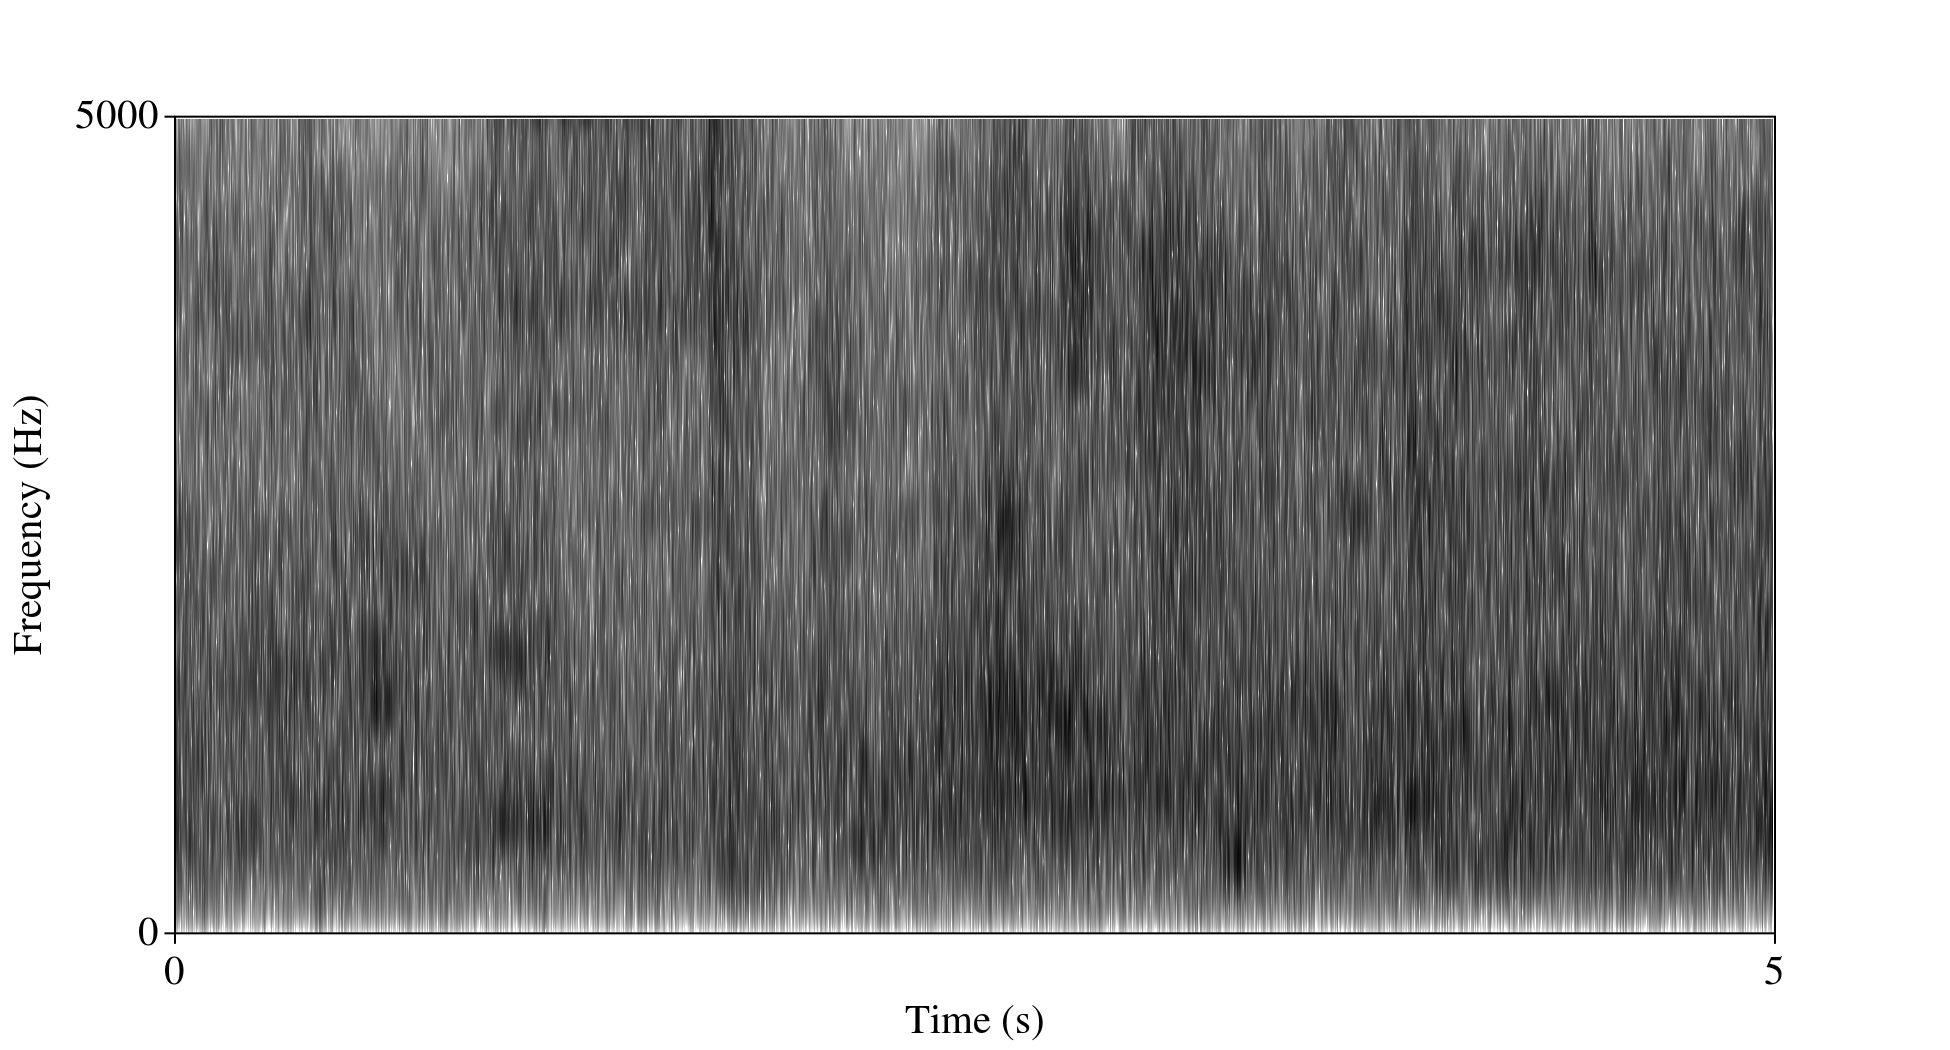
\includegraphics[width=0.9\textwidth]{figure/spctgrm-fac-background.png}
  \caption{Factory background noise.}
  \label{fig:fac-bkgrnd}
\end{subfigure}
\caption{Example spectograms of the first five seconds of the background noise tracks.}
\label{fig:bkgrnd-noises}
\end{figure}

Yet simply because a sound may be ``masked'' does not necessarily imply that the voice is not heard or understood.  There are a number of methods used by the auditory system to overcome the masking and understand the voice; this process is termed ``release from masking'' (\cite{middlebrooks:17}).  One such method, binaural hearing, uses both ears to tease apart the different sources, due to the very small temporal difference that occurs when different sound sources reach each ear.  
In this example, it is easy to see that energetic and informational masking are not strictly limited to masking separate ``lower'' and ``higher'' processes (\cite{durlach:06}).
The use of binaural hearing is an example of a ``higher'' process used for a release from energetic masking, as it necessarily requires signals from both ears to be interpreted (\cite{hirsh:47}). Binaural hearing is basically making use of the spatial directionality of the noise(s) from the listener to separate the different sources (\cite{bregman:94}).

Other methods of release from energetic masking include recognizing the difference between the fundamental frequency and timbre of two different sources, as well as making note of acoustic transitions: ``when [a] sound...changes its properties gradually, [it] is likely to be heard as a single changing sound.  However, when [it] changes...abruptly, [it] tends to be treated as a newly arriving sound, this tendency increasing with the abruptness of the change.'' (\cite{bregman:94}, 5).  Fundamental frequency (F0) has been shown to be an effective tool to presumably inpterpret the location of harmonics, and parse apart different sources (eg. two separate, simultaneous vowels with different F0s, \cite{bird:98}). There are many other proposed methods to release masking that the auditory system uses, particularly among informational masking (\cite{middlebrooks:17}), but these are beyond the scope of this project.


\subsection{Human Recognition Performance of Speech in Noise}

Eventually, however, with enough background noise and masking, the methods listed above for releasing the masking will fail and recognition will begin to break down.  Under the most simple conditions to measure, steady-state noise, (\cite{ding:13}) report that, when listening to speech in noise, human self reported intelligibility ratings don't drop significantly until the SNR reaches approximately -3 dB, where intelligibility drops to about 55\%, and it doesn't hit near floor level (0\%) until -9 db SNR.

This subjective measure is backed by a study performed by \cite{gilbert:13}, who used the PRESTO corpus (\cite{garofolo:93}) to test sentence intelligibility among 121 native English speakers.  \cite{gilbert:13} found that - similar to \cite{ding:13} - that the median score (at the 50th percentile) of speech with a -3dB SNR had about 55\% accuracy.  At +3 dB SNR, the 50th percentile increased to approximately 88\% accuracy.

\cite{ding:13} does however comment that there was great inter-speaker variation among the subjective measures of their perceived intelligibility of an utterance, and this is also supported by \cite{gilbert:13}'s results. They showed that, averaging over all SNR conditions (-5, -3, 0, +3), the variability between speakers had a range of almost 36\%; a retest performed with a subgroup of the original participants on the same dataset yielded a similar (~34\%) range of variability in accuracy.  

\cite{francis:10} discusses about how listening to speech in background noise places extra demands on working memory, as does listening to degraded speech (\cite{francis:09}).  The diversion of working memory to acoustic processing can be particularly detrimental to performance when simultaneously working on other computation, e.g. syntactic and semantic parsing (\cite{caplan:99}), such as in a phrase or sentence recognition. \cite{tamati:13} tested a group of high-performance against a separate group of low-performance hearers of speech in noise on several different working and short term memory tasks.  Not surprisingly, the group of listeners who are able to better hear speech in noise also perform statistically better on the working memory tasks.  This is by no means the only indicator of perceptual performance.

\cite{mattys:12} briefly discusses the concept of perceptual learning, which asserts that one can learn to accomodate a particular adverse condition (eg. background noise, signal distortion, etc.) with practice in that area.  Learning will be less effective in cases which the degradation is variable or unpredicatble between trials, such as with unpredictable background noise.  The present study is designed with this in mind, that the speech with the background noises will be presented in a random order, and since the background noise varies, it cannot be assumed or predicted from one sentence to the next.

Although there is expected to be a great amount of variability between subjects, the results from the \cite{ding:13} and \cite{gilbert:13} studies indicate that the average SNR for the highest noise condition from the data collected and described in Chapter 2\ref{chapter2}\footnote{The 80 dB noise condition yielded approximately +6dB SNR} is over 9 dB SNR above the 50\% intelligibility threshold at -3 db SNR given by these two studies.  It is unlikely that listeners will encounter much masking in the collected noisy speech that won't be overcome.

Due to this, two additional participants were rerun with lower SNRs, explained more in Section \ref{expt2}.

%Experiment redo

% Rediscuss these (learning directly above, cover briefly) in brief background when introducing secondary studies)
%PERCEPTUAL LEARNING AS IMPETUS FOR READING TRAINING TASK
%FREQUENCY as release of energetic masking AS IMPETUS FOR COMBINATION STIMULI


\section{Experiment 2: Human Speech Perception in Noise}
\label{expt2}

After analysing the results from a few pilot runs, it was deemed that the speech collected at the mouth in the noisy background described in Chapter \ref{chapter2} was too easily recognizeable for human listeners; i.e. the SNR ratio was not low enough, as explained in Section \ref{ch2:limitations}.  After additional stimuli were gathered (explained below in Section \ref{chap4:methods:stimuli}), a human speech perception experiment was run on the data collected in the first experiment in order to better understand and compare the ability of the auditory system to accurately comprehend the speech with a noisy background, and the speech distorted by passage through the speaker's head, and then modified to become more intelligible.  To act as a control, participants would also listen to normal, clean speech.

\subsection{Stimuli Generation}
\label{chap4:methods:stimuli}

To remedy the problem of the noisy speech being \textit{too} intelligible and having a high SNR, two additional participants (one male, one female) were recorded following the procedure in the first task (cf. Chapter \ref{chapter2}).  The list of stimuli was increased to 80 sentences (eight Harvard Sentence lists\footnote{This included the previous three lists, 14, 28, and 57, as well as lists 21, 29, 37, 53, and 68. These additional lists were pseudo-randomly chosen, as were the original three lists, to contain words that would be readily recognizeable by the participant population.}) to provide more reaction data from this present experiment.  

To increase the SNR, the directional microphone was pointed away from the mouth of the participant, and directed toward the loudspeaker (see fig. \ref{fig:overallSetUp_new}).  
%
\begin{wrapfigure}{r}{0.5\textwidth}
\centering
  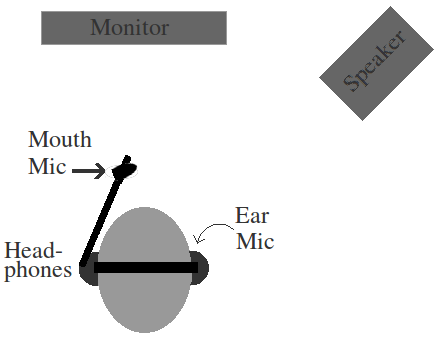
\includegraphics[width=0.45\textwidth]{figure/overallSetUp_new.png}
  \caption{This is the same setup as described in Chapter \ref{chapter2}, except that the microphone is facing the loudspeaker, rather than the participant's mouth.}
  \label{fig:overallSetUp_new}
\end{wrapfigure}
%
This, of course, results in some of the limitations outlined in section \ref{ch2:limitations} in Chapter 2; for example, simply pointing the mouth microphone toward the loudspeaker, rather than increasing the noise, ignores the fact that the noise level inside the ear might increase as well with an increase in ambient noise.  Given the alternatives outlined in section \ref{ch2:limitations}, this was seen as the best available option.  Figures \ref{fig:spectNewMouthNoise} and \ref{fig:spectNewEarNoise} show the new noisy and ear recorded speech, respectively.
%
\begin{figure}
\begin{subfigure}{0.5\textwidth}
  \centering
  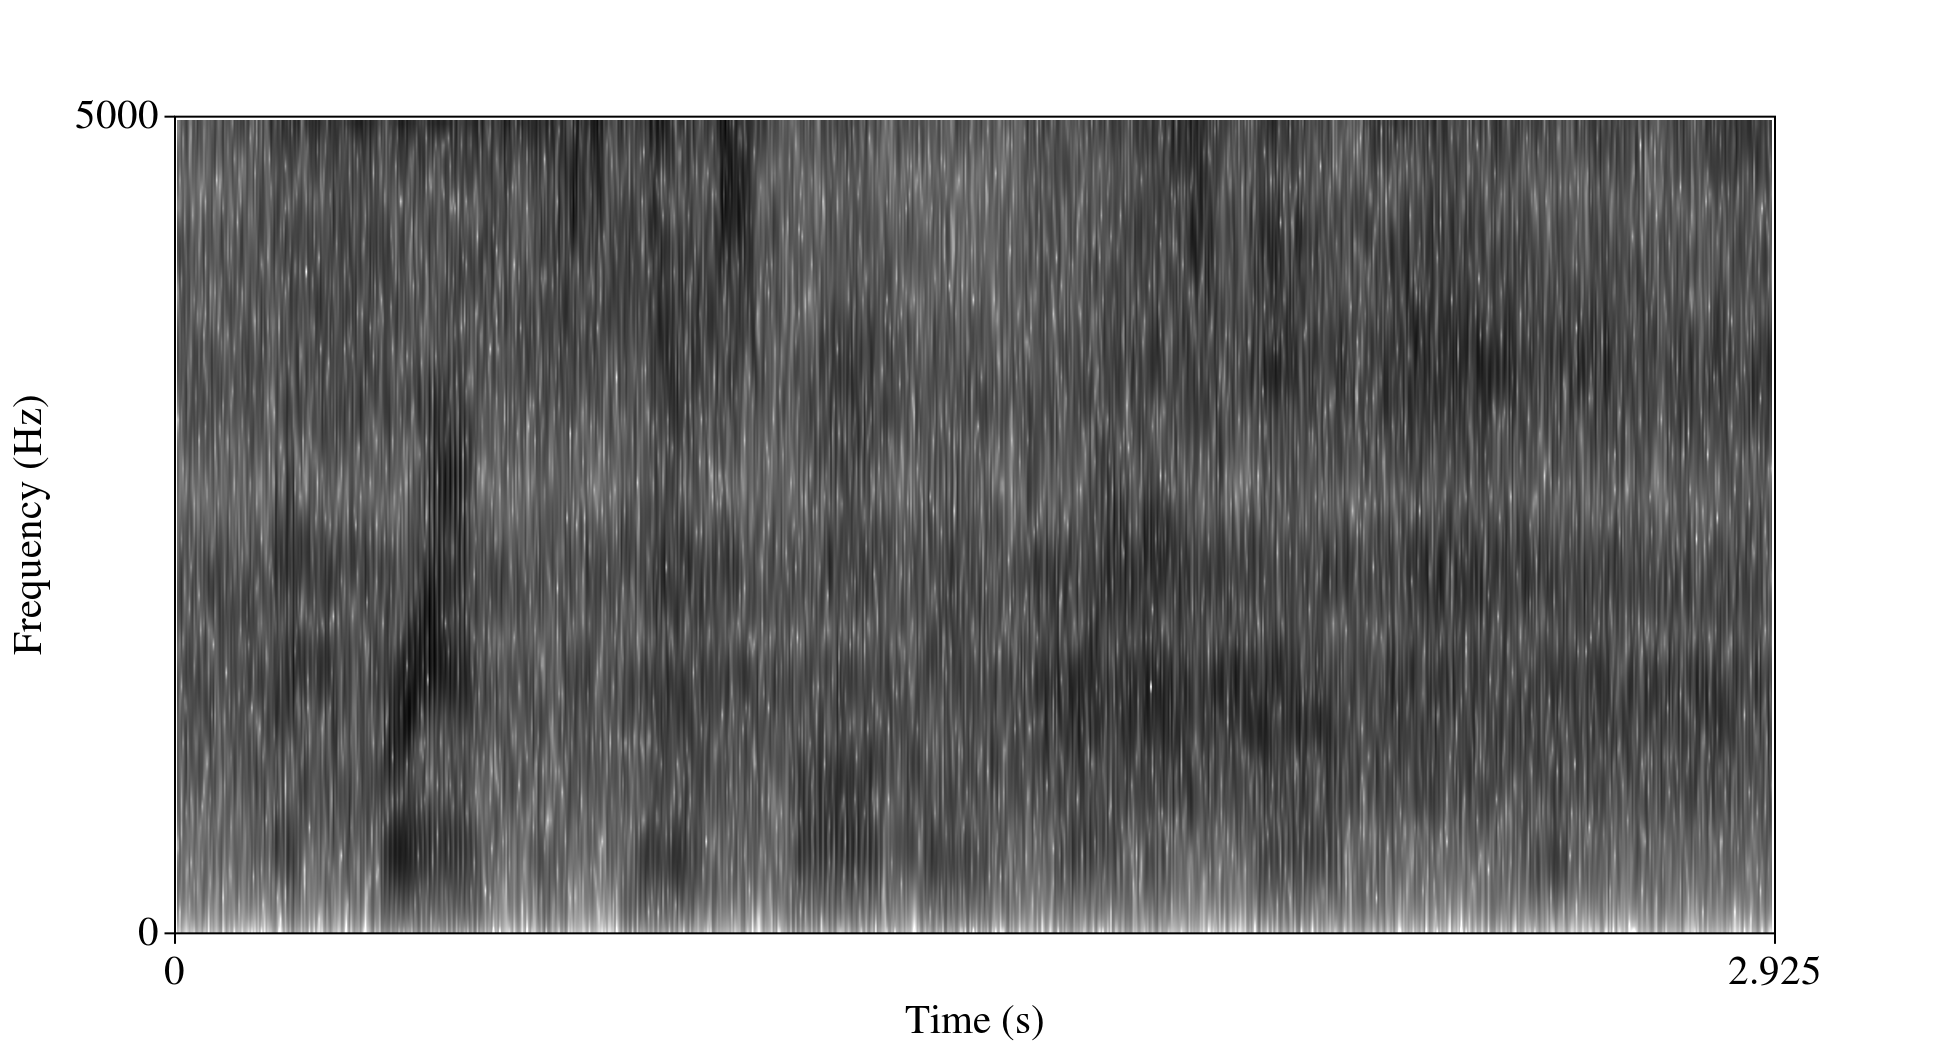
\includegraphics[width=0.9\textwidth]{figure/spectNewMouthNoise.png}
  \caption{New recording at the mouth with the microphone pointed toward the loudspeaker noise source.}
  \label{fig:spectNewMouthNoise}
\end{subfigure}
\begin{subfigure}{0.5\textwidth}
  \centering
  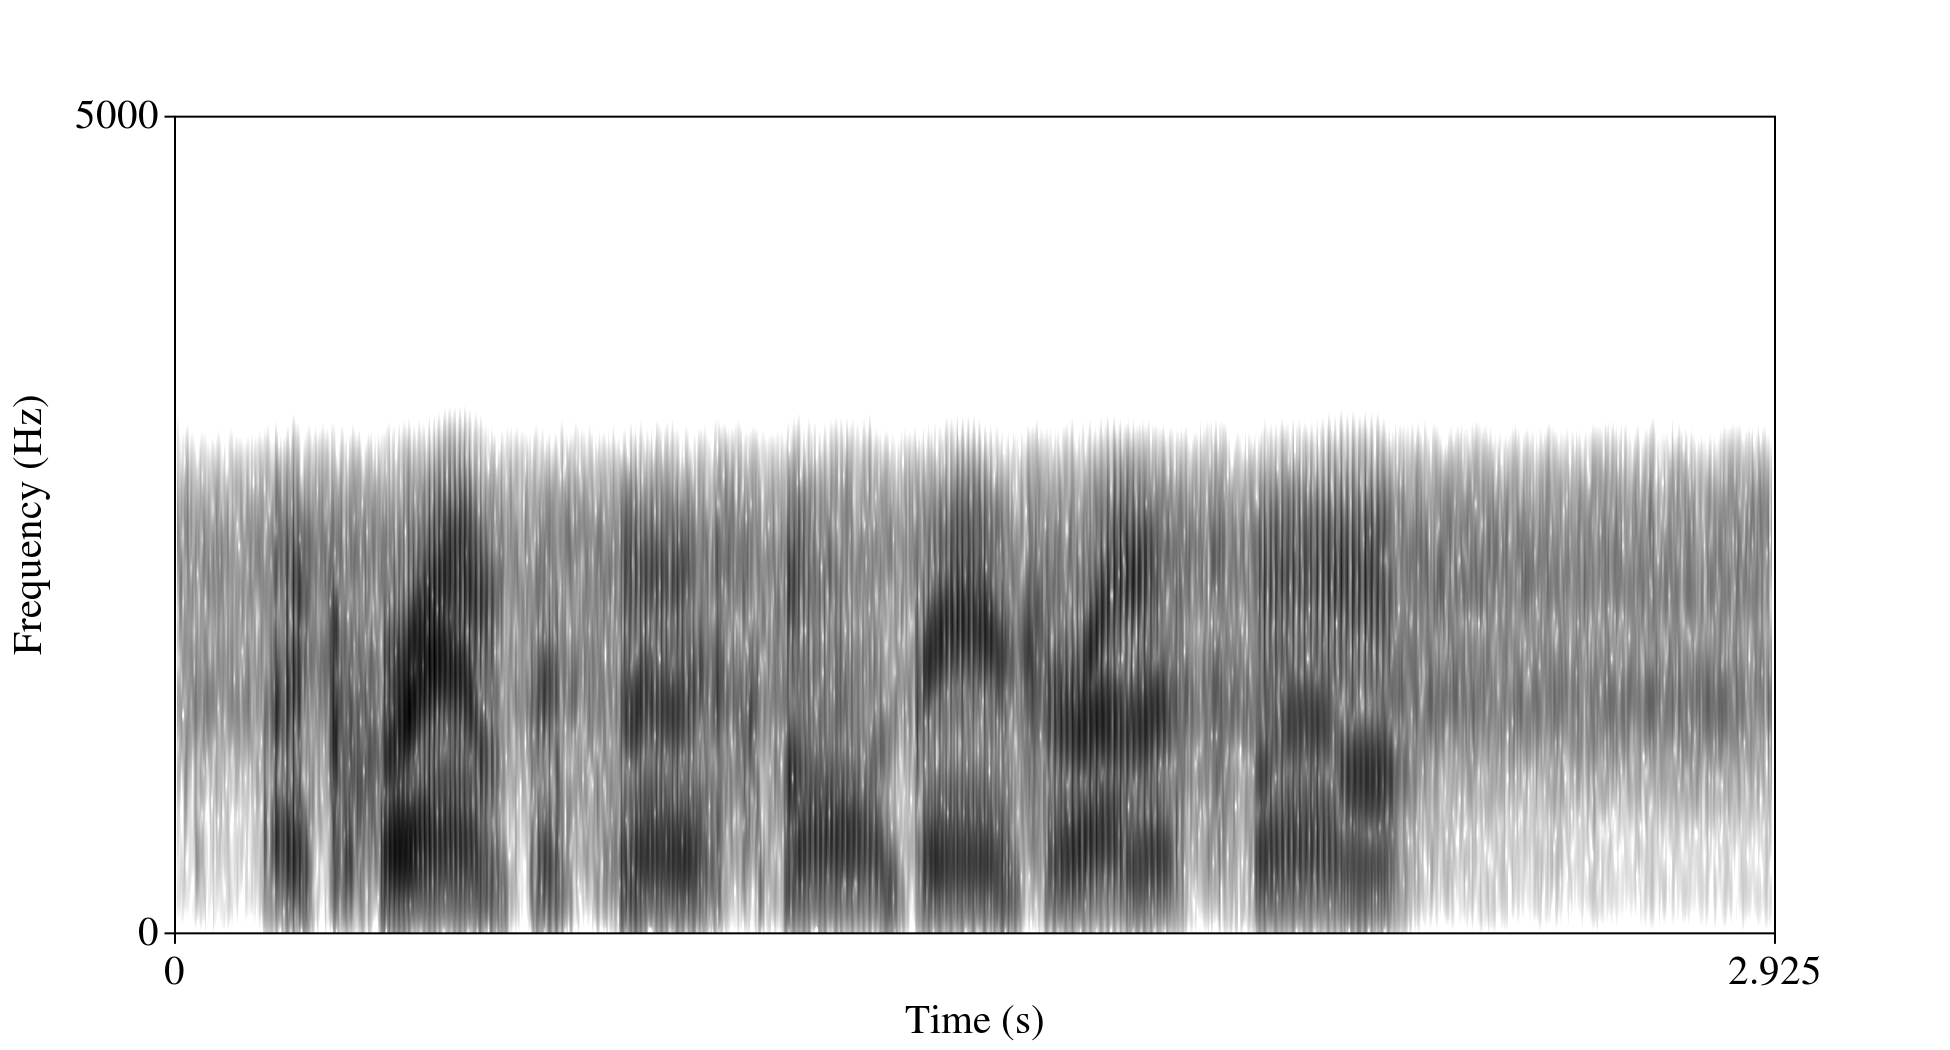
\includegraphics[width=0.9\textwidth]{figure/spectNewEarNoise.png}
  \caption{New recording at the ear; all recording conditions for the ear were the same as in the first group of recordings.}
  \label{fig:spectNewEarNoise}
\end{subfigure}
\caption{The sentence ``A cramp is no small danger on a swim'' spoken by the male speaker, recorded at the mouth (Fig. \ref{fig:spectNewMouthNoise}) with ``cafe'' noise, and simultaneously at the ear (Fig. \ref{fig:spectNewEarNoise})}
\end{figure}


Furthermore, due to the issue of the lack of noise, only one noise level condition was used - the highest available noise level (80 dB).  All previously used background noises were used for this data collection task as well.


\subsection{Design}
\label{chap4:methods:design}

The experiment had three factors - gender of speaker \textbf{x} microphone location \textbf{x} noise type - resulting in a 2x2x6 experiment.  There were two genders, two mic locations (recording at the ear, and at the mouth), and six noise types (bus, cafe, pedestrian, street, factory, and no noise (clean)).  Since the ability to understand speech in noise is quite variable between individuals, the design of this experiment was a within-subjects experiment.  This meant that each of the 2x2x6 (ie. 24) conditions needed to be seen by each participant.  The sessions that were re-recorded constituted 80 sentences, which allowed for three sentences in each of the 24 conditions, totalling 72 sentences used in the experiment.  The eight remaining sentences were used as a ``training'' set, intended to get the participants used to the task itself, rather than to acclimate them the type of speech that they would hear.

Since any given speaker could not hear the same sentence twice without introducing a confound, and since each sentence occurred in each of the 24 conditions, this necessitated the use of 24 co-balanced lists to ensure that each sentence was heard in every condition.  For example, sentences 1, 2, and 3 would occur in Factor \#1 (e.g. female speaker, mic at the mouth, with bus background noise) in co-balanced group \#1 for Participant \#1. Participant \#2 would see co-balanced group \#2, which placed sentences 1, 2, and 3 in Factor \#2 (e.g. female speaker, mic at the mouth, with cafe background noise).  For simplicity's sake, each grouping of three sentences would appear together in a given condition, and were not mixed up between the different co-balanced groups.  However, once the sentences are assigned to a particular condition, the order of presentation to the participants is randomized.

\subsection{Participants}

Twenty-four native speakers of English with self-reported normal hearing participated in the experiment. Each participant was placed into a separate co-balanced group, as specified in \ref{chap4:methods:design}.

\subsection{Equipment}

The experiment was conducted in a soundbooth with a pair of over-the-ear headphones.  The experiment used in-house developed software, and participants answers were typed into a computer whose monitor could be seen from inside the soundbooth.

\subsection{Procedure}
\label{hsp-main-procedure}

The participant was seated in the sound booth in front of a keyboard and computer monitor, with a pair of headphones, and were given a set of instructions. They were told that they would hear each utterance only once, and what they would hear was comprised of real English words, but may not constitute a ``complete'' sentence.  They were forewarned that many of the sentences they heard would be noisy and difficult to understand. They were instructed to write all words they heard, even if what was heard did not make syntactic sense, or if the words were not adjacent (e.g. if only the first and last word of the sentence was heard). They would be timed, with 18 seconds to type their response starting from the beginning of the soundfile and that their answer would be saved as is if they ran into the time limit, preventing them frrom typing more.

The participant was told that the first set of eight utterances they heard were part of a ``training'' set of eight utterances.  These were given to introduce the participants to the experiment and their task\footnote{The same eight sentences were heard by every participant}.  None of the utterances from the training set were used in the analysis.  Once completed with this initial set, participants were asked if they had any questions.  Afterwards they began the task in the soundbooth.  They would hear one of the sentences, and type their answer in a text box.  When finished with their answer, they would either click to advance to the next sentence, or, if they ran into the time limit, were prevented from modifying their answer, and were prompted to click another button to advance.  When finished with all 72 stimuli, the participant was given a brief questionnaire to fill out.  

After the experiment, the researcher would double check participant answers for correct spelling.  Only obvious errors were modified (e.g. `teh' to `the', `crakers' to `crackers', `mantle' to `mantel'), while ambiguous errors were left as-is (e.g. `blo' was not changed to `block', `finde' was not changed to `fine').  Numbers were also lexicalized (e.g. `30' to `thirty').  Punctuation was removed for ease of analysis and calculation of word error rate.  Exact responses are given by each participant can be found in Appendix F\ref{appendixF}.


\section{Results}



The word error rate (WER) for each (spell-checked) response for each participant was calculated. The code for the WER calculation can be found in Appendix F\ref{appendix?}

A 3-way, within-subjects ANOVA was performed with the collected data, 72 sentences each from 24 participants. Factors included the gender of the speaker (of the stimulus) with two levels, male and female, the location of the recording microphone with two levels, at the mouth and at the ear, and the background noise type with six levels, bus noise, cafe noise, pedestrian noise, factory noise, street noise, and no noise.  There was no significant 3-way interaction between speaker gender, noise type, and mic location, as can be seen in Tables \ref{tab:anova1_by_subj} and \ref{tab:anova1_by_item}. Two, two-way interactions were significant, speaker gender by mic location, and noise-type by mic location.  The main effects of all three factors were also significant (cf. Tables \ref{tab:anova1_by_subj} and \ref{tab:anova1_by_item}).

% latex table generated in R 3.4.0 by xtable 1.8-2 package
% Sun Jun 25 07:26:25 2017
\begin{table}[ht]
\centering
\begin{tabular}{lrrrrl}
  \hline
Effect & DFn & DFd & F & p & p$<$.05 \\ 
  \hline
speaker\_gender & 1.00 & 23.00 & 5.90 & 0.02 & * \\ 
  noise\_type & 5.00 & 115.00 & 70.59 & 0.00 & * \\ 
  mic\_location & 1.00 & 23.00 & 129.09 & 0.00 & * \\ 
  speaker\_gender:noise\_type & 5.00 & 115.00 & 0.58 & 0.72 &  \\ 
  speaker\_gender:mic\_location & 1.00 & 23.00 & 14.87 & 0.00 & * \\ 
  noise\_type:mic\_location & 5.00 & 115.00 & 47.97 & 0.00 & * \\ 
  speaker\_gender:noise\_type:mic\_location & 5.00 & 115.00 & 1.70 & 0.14 &  \\ 
   \hline
\end{tabular}
\caption{ANOVA for by-subjects analysis of the three-factor, within-subjects experiment.} 
\label{tab:anova1_by_subj}
\end{table}
% latex table generated in R 3.4.0 by xtable 1.8-2 package
% Sun Jun 25 07:26:26 2017
\begin{table}[ht]
\centering
\begin{tabular}{lrrrrl}
  \hline
Effect & DFn & DFd & F & p & p$<$.05 \\ 
  \hline
speaker\_gender & 1.00 & 71.00 & 4.36 & 0.04 & * \\ 
  noise\_type & 5.00 & 355.00 & 100.88 & 0.00 & * \\ 
  mic\_location & 1.00 & 71.00 & 282.24 & 0.00 & * \\ 
  speaker\_gender:noise\_type & 5.00 & 355.00 & 0.56 & 0.73 &  \\ 
  speaker\_gender:mic\_location & 1.00 & 71.00 & 17.38 & 0.00 & * \\ 
  noise\_type:mic\_location & 5.00 & 355.00 & 65.00 & 0.00 & * \\ 
  speaker\_gender:noise\_type:mic\_location & 5.00 & 355.00 & 1.69 & 0.14 &  \\ 
   \hline
\end{tabular}
\caption{ANOVA for by-items analysis of the three-factor, within-subjects experiment.} 
\label{tab:anova1_by_item}
\end{table}



Mauchley's Test for Sphericity was conducted, both for the by-subjects and by-items ANOVAs.  Significant sphericity violations were found for the main effect of noise type, and the interaction of speaker gender and noise type, as can be seen in Tables \ref{tab:anova1_subj_sph_test} and \ref{tab:anova1_item_sph_test}. 

% latex table generated in R 3.4.0 by xtable 1.8-2 package
% Sun Jun 25 07:26:26 2017
\begin{table}[ht]
\centering
\begin{tabular}{lrrl}
  \hline
Effect & W & p & p$<$.05 \\ 
  \hline
noise\_type & 0.27 & 0.02 & * \\ 
  speaker\_gender:noise\_type & 0.62 & 0.76 &  \\ 
  noise\_type:mic\_location & 0.43 & 0.23 &  \\ 
  speaker\_gender:noise\_type:mic\_location & 0.59 & 0.69 &  \\ 
   \hline
\end{tabular}
\caption{Sphericity test for the by-subjects ANOVA.} 
\label{tab:anova1_subj_sph_test}
\end{table}
% latex table generated in R 3.4.0 by xtable 1.8-2 package
% Sun Jun 25 07:26:26 2017
\begin{table}[ht]
\centering
\begin{tabular}{lrrl}
  \hline
Effect & W & p & p$<$.05 \\ 
  \hline
noise\_type & 0.79 & 0.28 &  \\ 
  speaker\_gender:noise\_type & 0.67 & 0.02 & * \\ 
  noise\_type:mic\_location & 0.86 & 0.75 &  \\ 
  speaker\_gender:noise\_type:mic\_location & 0.86 & 0.71 &  \\ 
   \hline
\end{tabular}
\caption{Sphericity test for the by-items ANOVA.} 
\label{tab:anova1_item_sph_test}
\end{table}
% latex table generated in R 3.4.0 by xtable 1.8-2 package
% Sun Jun 25 07:26:26 2017
\begin{table}[ht]
\centering
\begin{tabular}{lrrl}
  \hline
Effect & GGe & p[GG] & p[GG]$<$.05 \\ 
  \hline
noise\_type & 0.63 & 0.00 & * \\ 
  speaker\_gender:noise\_type & 0.86 & 0.69 &  \\ 
  noise\_type:mic\_location & 0.77 & 0.00 & * \\ 
  speaker\_gender:noise\_type:mic\_location & 0.83 & 0.15 &  \\ 
   \hline
\end{tabular}
\caption{Sphericity corrections for the by-subjects ANOVA.} 
\label{tab:anova1_subj_sph_corr}
\end{table}
% latex table generated in R 3.4.0 by xtable 1.8-2 package
% Sun Jun 25 07:26:26 2017
\begin{table}[ht]
\centering
\begin{tabular}{lrrl}
  \hline
Effect & GGe & p[GG] & p[GG]$<$.05 \\ 
  \hline
noise\_type & 0.92 & 0.00 & * \\ 
  speaker\_gender:noise\_type & 0.87 & 0.71 &  \\ 
  noise\_type:mic\_location & 0.95 & 0.00 & * \\ 
  speaker\_gender:noise\_type:mic\_location & 0.95 & 0.14 &  \\ 
   \hline
\end{tabular}
\caption{Sphericity corrections for the by-subjects ANOVA.} 
\label{tab:anova1_item_sph_corr}
\end{table}


The sphericity tests for both by-subjects and by-items ANOVAs both returned with a change in the two way interaction between speaker gender and noise, it not being significant.  Noting the sphericity violations involving noise type, the data was viewed in the box plots in Figures \ref{fig:anova1_noise_boxplot}, \ref{fig:anova1_noiseXspkr_boxplot}, and \ref{fig:anova1_noiseXmic_boxplot}.  It can easily be noted that the conditions in which there was no background noise differ distinctly from the conditions in which there is background noise.


\begin{wrapfigure}{L}{0.75\textwidth}

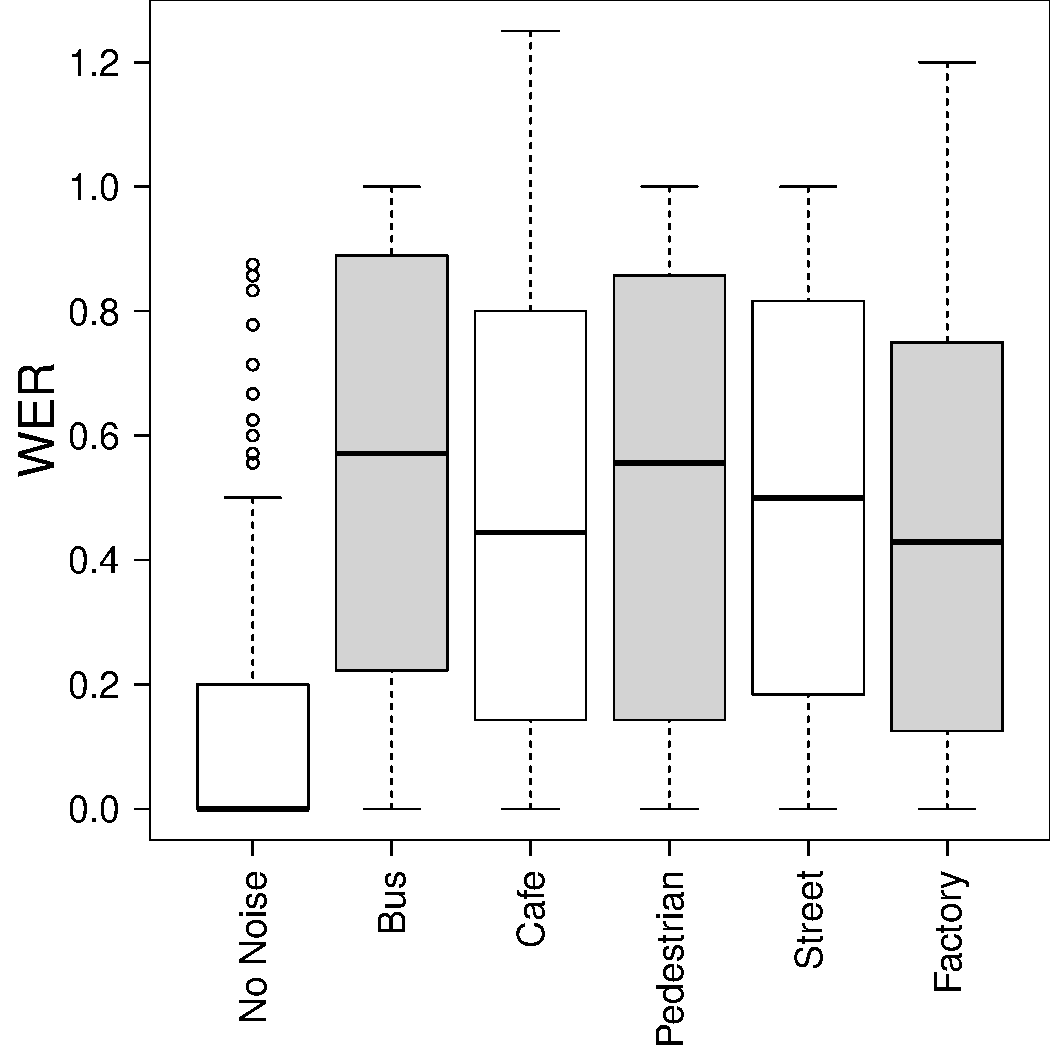
\includegraphics[width=\maxwidth]{figure/boxplot_noise-1} 

\caption{Boxplot displaying the average word error rate (WER) averaged over each participant for every noise type. WER is the variable on the y-axis, and noise type is on the x-axis.}
\label{fig:anova1_noise_boxplot}
\end{wrapfigure}

%\begin{wrapfigure}{L}{1\textwidth}
\begin{wrapfigure}{L}{0.75\textwidth}

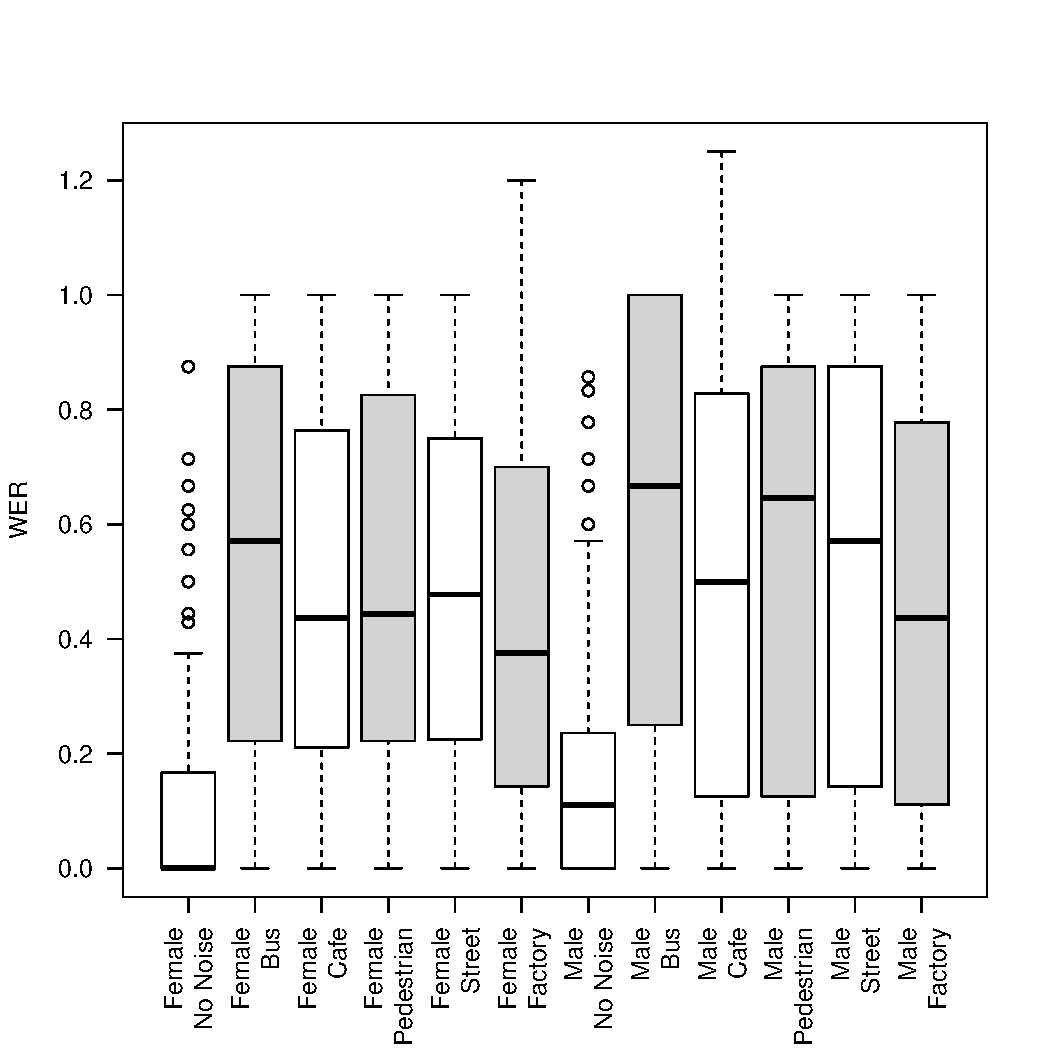
\includegraphics[width=\maxwidth]{figure/boxplot_noiseXspkr-1} 

\caption{Boxplot displaying the average word error rate (WER) averaged over each participant for the interaction of every noise type by the speaker gender. WER is the variable on the y-axis, and noise type by speaker gender is on the x-axis.}
\label{fig:anova1_noiseXspkr_boxplot}
\end{wrapfigure}

\begin{wrapfigure}{L}{0.75\textwidth}

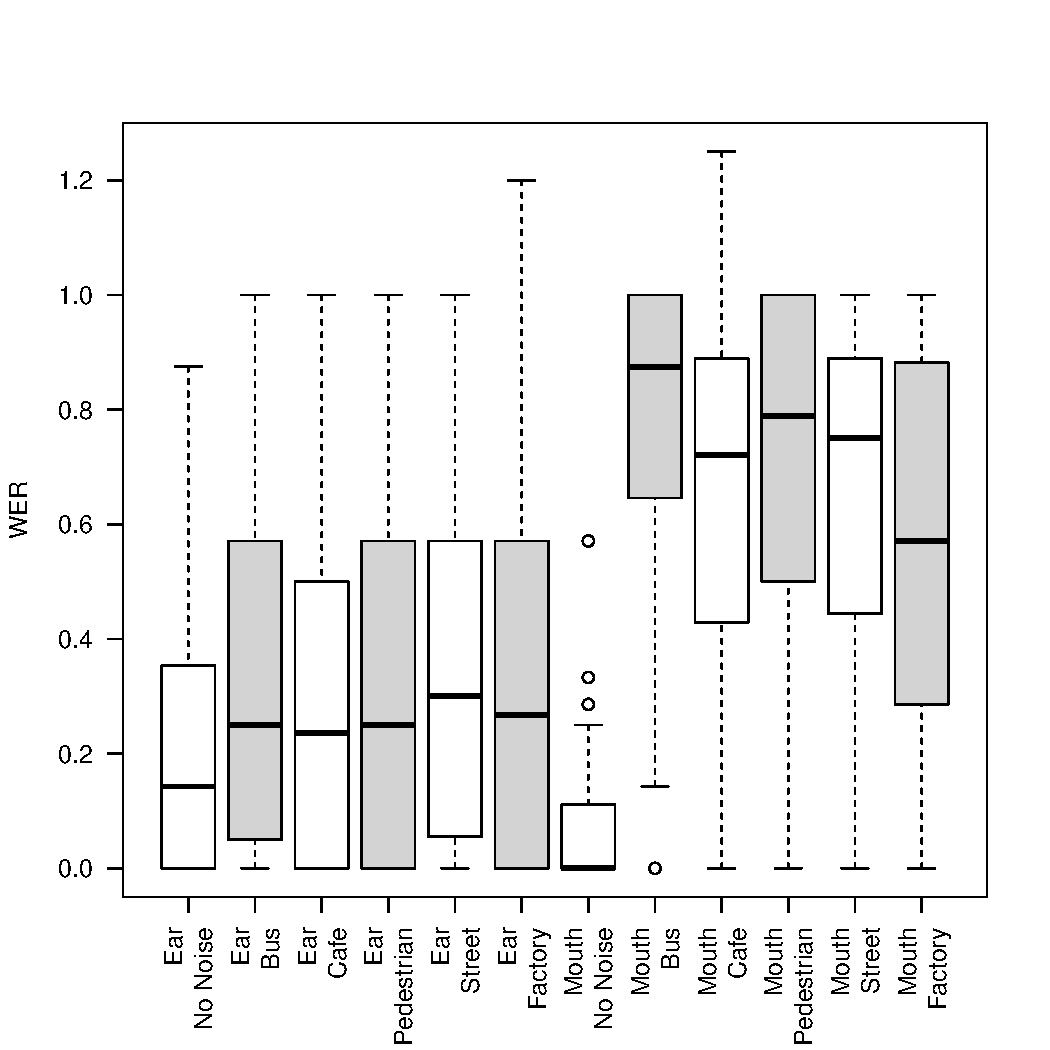
\includegraphics[width=\maxwidth]{figure/boxplot_noiseXmic-1} 

\caption{Boxplot displaying the average word error rate (WER) averaged over each participant for the interaction of every noise type by the mic location. WER is the variable on the y-axis, and noise type by mic location is on the x-axis.}
\label{fig:anova1_noiseXmic_boxplot}
\end{wrapfigure}

This is likely the root of the sphericity violations.  Since it there is a main effect of statistical difference in noise, and since the ``no noise'' condition is very apparently different from the rest, this condition was removed, and another ANOVA calculated to test for statistical difference only in noise conditions containing noise. 

% latex table generated in R 3.4.0 by xtable 1.8-2 package
% Sun Jun 25 07:26:26 2017
\begin{table}[ht]
\centering
\begin{tabular}{lrrrrl}
  \hline
Effect & DFn & DFd & F & p & p$<$.05 \\ 
  \hline
speaker\_gender & 1.00 & 23.00 & 5.17 & 0.03 & * \\ 
  noise\_type & 4.00 & 92.00 & 4.35 & 0.00 & * \\ 
  mic\_location & 1.00 & 23.00 & 185.74 & 0.00 & * \\ 
  speaker\_gender:noise\_type & 4.00 & 92.00 & 0.62 & 0.65 &  \\ 
  speaker\_gender:mic\_location & 1.00 & 23.00 & 13.41 & 0.00 & * \\ 
  noise\_type:mic\_location & 4.00 & 92.00 & 5.44 & 0.00 & * \\ 
  speaker\_gender:noise\_type:mic\_location & 4.00 & 92.00 & 1.44 & 0.23 &  \\ 
   \hline
\end{tabular}
\caption{ANOVA for by-subjects analysis of the three-factor, within-subjects experiment. The ``no noise'' condition was removed from the noise type factor, resulting in a 2x2x5 design.} 
\label{tab:anova1_by_subj}
\end{table}
% latex table generated in R 3.4.0 by xtable 1.8-2 package
% Sun Jun 25 07:26:27 2017
\begin{table}[ht]
\centering
\begin{tabular}{lrrrrl}
  \hline
Effect & DFn & DFd & F & p & p$<$.05 \\ 
  \hline
speaker\_gender & 1.00 & 71.00 & 3.67 & 0.06 &  \\ 
  noise\_type & 4.00 & 284.00 & 6.23 & 0.00 & * \\ 
  mic\_location & 1.00 & 71.00 & 436.86 & 0.00 & * \\ 
  speaker\_gender:noise\_type & 4.00 & 284.00 & 0.60 & 0.66 &  \\ 
  speaker\_gender:mic\_location & 1.00 & 71.00 & 16.48 & 0.00 & * \\ 
  noise\_type:mic\_location & 4.00 & 284.00 & 6.82 & 0.00 & * \\ 
  speaker\_gender:noise\_type:mic\_location & 4.00 & 284.00 & 1.41 & 0.23 &  \\ 
   \hline
\end{tabular}
\caption{ANOVA for by-items analysis of the three-factor, within-subjects experiment. The ``no noise'' condition was removed from the noise type factor, resulting in a 2x2x5 design.} 
\label{tab:anova1_by_item}
\end{table}



\section{Initial Discussion}

*Some participants noted that the computer screen was a distraction to their ability to perceive the utterances. Cite \cite{mattys:13} regarding ``Reduced Attentional Capacity'', briefly touched on in the Background/lit review.


\section{Follow-up Pilot Experiments}

To expound on the previous study, two additional pilot studies were performed to give insights into possible future directions.  The impetus for the first study was the study performed by \cite{bird:98}, which demonstrated that the fundamental frequency (F0) was a tool used by the auditory system to separate a desired source from masking noise.  This follow up proposes to recombine the very clear, lower frequencies with the ``noisy'' upper frequencies recorded at the mouth.  The hypothesis is that the auditory system will use the clear fundamental frequency harmonic information in the lower frequencies to extract the upper harmonics out of the noise.  Accuracy is predicted to improve over that of the low-pass filtered, ``muffled'', ear speech (which many participants subjectively observed to be annoying and difficult to understand), as more high frequency information will be present and available for participants.  This speech will sacrifice the advantage of being completely ``noise-free'', to sound more natural.  Additionally, since the ear-recorded speech consists of very clean harmonics, it is hypothesized that this speech, combined with the higher frequency mouth recorded speech in the noise-free condition, will perform equal to the plain ``clean'' speech condition. This will be referred to as the ``F0'' study.

The second follow-up experiment was based on the concept of ``perceptual learning'' discussed earlier.  This presumes that the auditory system can learn to adapt to understand speech in a degraded signal better over time.  According to \cite{mattys:12}, significant learning can occur with even a small number of training trials. While also intuitive, \cite{davis:05} demonstrate that during training, successful recognition of a degraded signal will help one recognize a similar signal more than unsuccessful recognition of a degraded signal.  Based on these findings, a short story was read and recorded from inside the ear canal for the participants in this follow up study to listen to prior to completing the experiment itself.  Since the type of distortion from the ear recorded signal is regular and predictable, it is hypothesized that perceptual learning will take place (unlike with the unpredictable speech in noise c.f. \cite{peelle:05}), and those who have listened to the training story will perform better on ear-recorded speech than those who had not. This will be referred to as the ``perceptual learning'' study.


\subsection{``F0'' Study Methods}
\label{F0-methods}

The stimuli used for this study consisted of the exact same sentences produced by the exact same speakers.  No modification was performed to the sentences recorded at the mouth.  For the sentences recorded at the ear, the same modifications as before (pre-emphasis, lowpass filtering\footnote{Lowpass filtered allowing 0-2500Hz, with a 500 Hz slope}, and a second pre-emphasis), but this time the simultaneously recorded speech from the mouth was filtered and combined with the ear-recorded speech.  The speech from the mouth was bandpass filtered between 3000Hz and 8000Hz, with a 500Hz slope.  This allowed for an overlap of the frequencies from the mouth-recorded speech and the lowpass filtered ear-recorded speech.  The two signals were converted to a stereo signal, and then combined into a mono signal.  This resulted in clean speech below approximately 2700Hz, and noisy speech above approximately 2700Hz, as seen in Figure \ref{fig:combined-signal}.
%
\begin{wrapfigure}{r}{0.5\textwidth}
\centering
  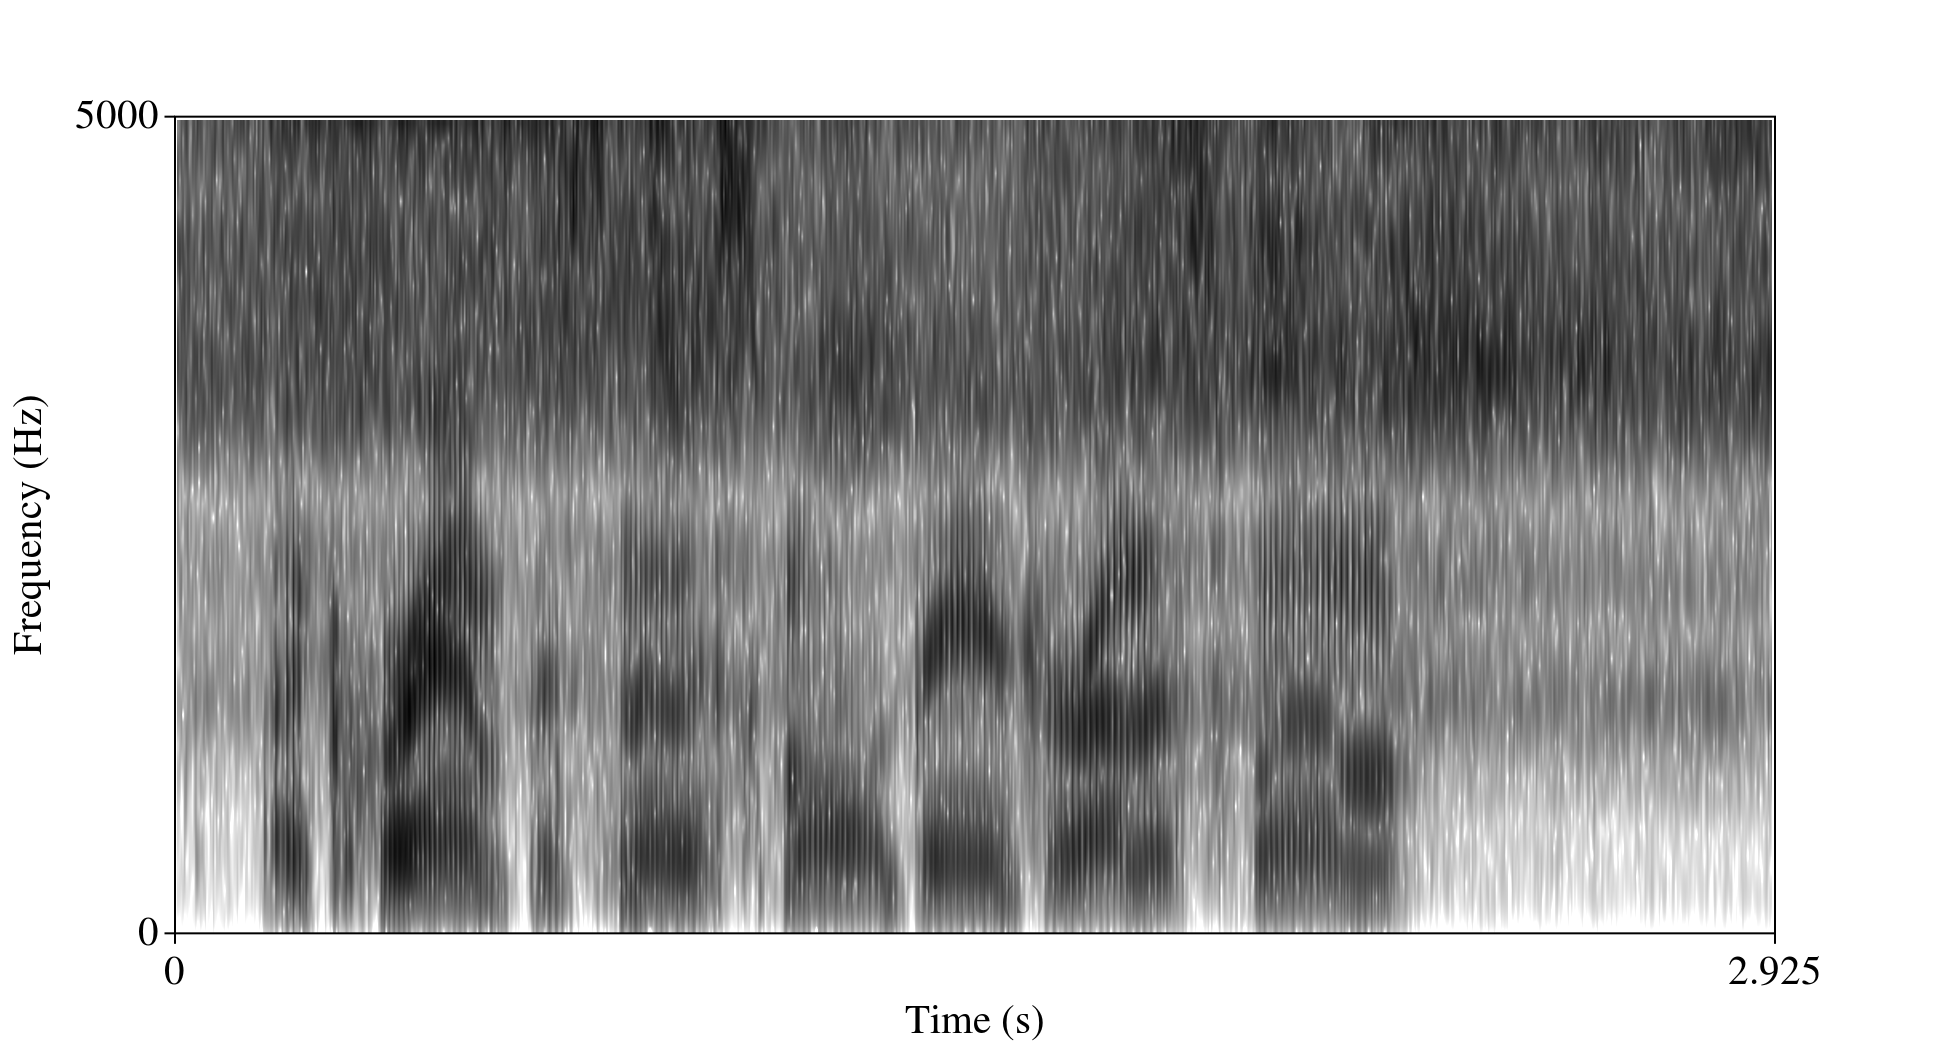
\includegraphics[width=0.45\textwidth]{figure/combined-signal.png}
  \caption{A spectrogram of the sentence ``A cramp is no small danger on a swim''.  The low-pass filtered ear-recorded signal was combined with the simultenous [noisy] mouth speech, which was bandpass filtered at a higher frequency.}
  \label{fig:combined-signal}
\end{wrapfigure}
%

Four native speakers of English with self-reported normal hearing participated in this study.  The design and procedure of this experiment was exactly the same as the initial perception experiment, save the alteration in modifications performed on the ear-recorded stimuli.


\subsection{``F0'' Study Results}


\subsection{``Perceptual Learning'' Methods}

For this study, a new speaker was recorded from the ear canal (with the same set-up as all previous recordings) reciting the short story ``Peter Rabbit'', by Beatrix Potter.  The recorded had a total length of approximately 5 minutes and 13 seconds.  The recorded story underwent the same transformations as the ear-recorded stimuli (pre-emphasis, lowpass filtering\footnote{Lowpass filter of 0-2500Hz with a 500Hz slope.}, and pre-emphasis).

There were four native speakers of English with self-reported normal hearing who participated in this follow up study.  They were first presented with a transcript of the story, and asked to listen to the audio and read along.  This offers ample chance for ``successful'' recognition of the degraded ear-recorded signal (cf. \cite{davis:05}).  After the reading session, the participants conducted the experiment as was done in the other studies mentioned in Sections \ref{hsp-main-procedure} and \ref{F0-methods}.

\subsection{``Perceptual Learning'' Results}



\subsection{Global Discussion}





\bibliographystyle{apa}
\bibliography{DissRefs.bib}
\end{document}
